\ifdefined\maindoc\else
% typesetting this chapter as a standalone document
\def\doctitle{Inverse Simulation}
% starting definitions for both the main document and stand-alone chapters
\documentclass{book}

\def\mech{artisynth.core.mechmodels}
\def\mgeo{maspack.geometry}

% Add search paths for input files
\makeatletter
\def\input@path{{../}{../../}{../texinputs/}}
\makeatother

\usepackage{amsmath}
\usepackage{framed}
%%
%% Default settings for artisynth
%%
\NeedsTeXFormat{LaTeX2e}
%%\ProvidesPackage{artisynthDoc}[2012/04/05]

\usepackage[T1]{fontenc}
\usepackage[latin1]{inputenc}
\usepackage{listings}
\usepackage{makeidx}
\usepackage{latexml}
\usepackage{graphicx}
\usepackage{framed}
\usepackage{booktabs}
\usepackage{color}

\newcommand{\pubdate}{\today}
\newcommand{\setpubdate}[1]{\renewcommand{\pubdate}{#1}}
\newcommand{\code}[1]{{\tt #1}}

\iflatexml
\usepackage{hyperref}
\setlength\parindent{0pt} 
\else
%% then we are making a PDF, so include things that LaTeXML can't handle: 
%% docbook style, \RaggedRight
\usepackage{ifxetex}
\usepackage{xstring}
\usepackage{pslatex} % fixes fonts; in particular sets a better-fitting \tt font

\usepackage[most]{tcolorbox}
\definecolor{shadecolor}{rgb}{0.95,0.95,0.95}
\tcbset{
    frame code={}
    center title,
    left=0pt,
    right=0pt,
    top=0pt,
    bottom=0pt,
    colback=shadecolor,
    colframe=white,
    width=\dimexpr\textwidth\relax,
    enlarge left by=0mm,
    boxsep=0pt,
    arc=0pt,outer arc=0pt,
}%

\usepackage[A4]{artisynth_papersize}
%\usepackage[letter]{artisynth_papersize}
\usepackage[hyperlink]{asciidoc-dblatex} 

%\usepackage{verbatim}
\usepackage{ragged2e}
\setlength{\RaggedRightRightskip}{0pt plus 4em}
\RaggedRight
\renewcommand{\DBKpubdate}{\pubdate}
\renewcommand{\DBKreleaseinfo}{}
\fi

% set hypertext links to be dark blue:
\definecolor{darkblue}{rgb}{0,0,0.8}
\definecolor{sidebar}{rgb}{0.5,0.5,0.7}
\hypersetup{colorlinks=true,urlcolor=darkblue,linkcolor=darkblue,breaklinks=true}

%%%%%%%%%%%%%%%%%%%%%%%%%%%%%%%%%%%%%%%%%%%%%%%%%%%%%%%%%%%%%%%%%%%%%%%%%%%%%
%
% Define macros for handling javadoc class and method references
%
%%%%%%%%%%%%%%%%%%%%%%%%%%%%%%%%%%%%%%%%%%%%%%%%%%%%%%%%%%%%%%%%%%%%%%%%%%%%%
\makeatletter

% macro to enable line break if inside a PDF file
\def\pdfbreak{\iflatexml\else\\\fi}

% code inspired by http://stackoverflow.com/questions/2457780/latex-apply-an-operation-to-every-character-in-a-string
\def\removeargs #1{\doremoveargs#1$\wholeString\unskip}
\def\doremoveargs#1#2\wholeString{\if#1$%
\else\if#1({()}\else{#1}\taketherest#2\fi\fi}
\def\taketherest#1\fi
{\fi \doremoveargs#1\wholeString}

% Note: still doesn't work properly when called on macro output ...
% i.e., \dottoslash{\concatnames{model}{base}{foo}} fails 
\def\dottoslash #1{\dodottoslash#1$\wholeString\unskip}
\def\dodottoslash#1#2\wholeString{\if#1$%
\else\if#1.{/}\else{#1}\fi\dottaketherest#2\fi}
\def\dottaketherest#1\fi{\fi \dodottoslash#1\wholeString}

\def\hashtodot #1{\dohashtodot#1$\wholeString\unskip}
\def\dohashtodot#1#2\wholeString{\if#1$X%
\else\if#1\#{.}\else{#1}\fi\hashtaketherest#2\fi}
\def\hashtaketherest#1\fi{\fi \dohashtodot#1\wholeString}

%\dollartodot{#1} does the same thing as \StrSubstitute[0]{#1}{\$}{.}
% from the packahe xstring. We define \dollartodot instead because
% LaTeXML does not implement xstring.
%
% Note that for the substituion to work, we need \ifx instead of \if,
% since otherwise escaped characters won't work properly:
% if #1 = \$, then \if#1* seems to compare '\' and '$' (and output '*'),
% rather than comparing '$' to '*'
\def\dollartodot #1{\dodollartodot#1*\wholeString\unskip}
\def\dodollartodot#1#2\wholeString{\ifx#1*%
\else \ifx#1\${.}\else{#1}\fi\dollartaketherest#2\fi}
\def\dollartaketherest#1\fi{\fi \dodollartodot#1\wholeString}

% concatenates up to three class/method names together, adding '.' characters
% between them. The first and/or second argument may be empty, in which case
% the '.' is omitted. To check to see if these arguments are empty, we
% use a contruction '\if#1@@', which will return true iff #1 is empty
% (on the assumption that #1 will not contain a '@' character).
\def\concatnames
#1#2#3{\if#1@@\if#2@@#3\else #2.#3\fi\else\if#2@@#1.#3\else#1.#2.#3\fi\fi}

\newcommand{\javabase}{}
\newcommand{\setjavabase}[1]{\renewcommand{\javabase}{#1}}

\def\artisynthDocBase{@ARTISYNTHDOCBASE}

\iflatexml
\def\ifempty#1{\def\temp{#1}\ifx\temp\empty}%
\newcommand{\artisynthManual}[3][]{%
   \ifempty{#1}
      \href{@ARTISYNTHDOCBASE/#2/#2.html}{#3}%
    \else
      \href{@ARTISYNTHDOCBASE/#1/#2.html}{#3}%
    \fi
}
\else
\newcommand{\artisynthManual}[3][]{%
\href{https://www.artisynth.org/@ARTISYNTHDOCBASE/#2.pdf}{#3}}
\fi

%\href{@ARTISYNTHDOCBASE/#2/#2.html}{#3}}



\newcommand{\javaclassx}[2][]{%
% Includes code to prevent an extra '.' at the front if #1 is empty. It
% works like this: if '#1' is empty, then '#1.' expands to '.', and so 
% '\if#1..' will return true, in which case we just output '#2'.
\href{@JDOCBEGIN/\concatnames{\javabase}{#1}{#2}@JDOCEND}{#2}}
\newcommand{\javaclass}[2][]{%
\href{@JDOCBEGIN/\concatnames{}{#1}{#2}@JDOCEND}{\dollartodot{#2}}}
\newcommand{\javaclassAlt}[2]{%
\href{@JDOCBEGIN/\concatnames{}{}{#1}@JDOCEND}{#2}}

\newcommand{\javamethodArgsx}[2][]{%
\href{@JDOCBEGIN/\concatnames{\javabase}{#1}{#2}@JDOCEND}{#2}}
\newcommand{\javamethodArgs}[2][]{%
\href{@JDOCBEGIN/\concatnames{}{#1}{#2}@JDOCEND}{#2}}
\newcommand{\javamethodAlt}[2]{%
\href{@JDOCBEGIN/\concatnames{}{}{#1}@JDOCEND}{#2}}
\newcommand{\javamethodAltx}[2]{%
\href{@JDOCBEGIN/\concatnames{\javabase}{}{#1}@JDOCEND}{#2}}

\newcommand{\javamethodNoArgsx}[2][]{%
\href{@JDOCBEGIN/\concatnames{\javabase}{#1}{#2}@JDOCEND}{\removeargs{#2}}}
\newcommand{\javamethodNoArgs}[2][]{%
\href{@JDOCBEGIN/\concatnames{}{#1}{#2}@JDOCEND}{\removeargs{#2}}}

\newcommand{\javamethod}{\@ifstar\javamethodNoArgs\javamethodArgs}
\newcommand{\javamethodx}{\@ifstar\javamethodNoArgsx\javamethodArgsx}

%%%%%%%%%%%%%%%%%%%%%%%%%%%%%%%%%%%%%%%%%%%%%%%%%%%%%%%%%%%%%%%%%%%%%%%%%%%%%
%
% Define macros for sidebars
%
%%%%%%%%%%%%%%%%%%%%%%%%%%%%%%%%%%%%%%%%%%%%%%%%%%%%%%%%%%%%%%%%%%%%%%%%%%%%%

\iflatexml
\newenvironment{sideblock}{\begin{quote}}{\end{quote}}
\else
\usepackage[strict]{changepage}
\definecolor{sidebarshade}{rgb}{1.0,0.97,0.8}
\newenvironment{sideblock}{%
    \def\FrameCommand{%
    \hspace{1pt}%
    {\color{sidebar}\vrule width 2pt}%
    %{\vrule width 2pt}%
    {\color{sidebarshade}\vrule width 4pt}%
    \colorbox{sidebarshade}%
  }%
  \MakeFramed{\advance\hsize-\width\FrameRestore}%
  \noindent\hspace{-4.55pt}% disable indenting first paragraph
  \begin{adjustwidth}{}{7pt}%
  %\vspace{2pt}\vspace{2pt}%
}
{%
  \vspace{2pt}\end{adjustwidth}\endMakeFramed%
}
\fi

\iflatexml
\newenvironment{shadedregion}{%
  \definecolor{shadecolor}{rgb}{0.96,0.96,0.98}%
  \begin{shaded*}%
% Put text inside a quote to create a surrounding blockquote that
% will properly accept the color and padding attributes
  \begin{quote}%
}
{%
  \end{quote}%
  \end{shaded*}%
}
\else
\newenvironment{shadedregion}{%
  \definecolor{shadecolor}{rgb}{0.96,0.96,0.98}%
  \begin{shaded*}%
}
{%
  \end{shaded*}%
}
\fi

% Wanted to create a 'listing' environment because lstlisting is
% tedious to type and because under latexml it may need
% some massaging to get it to work properly. But hard to do
% because of the verbatim nature of listing
%\iflatexml
%\newenvironment{listing}{\begin{lstlisting}}{\end{lstlisting}}%
%\else
%\newenvironment{listing}{\begin{lstlisting}}{\end{lstlisting}}%
%\fi

\iflatexml\else
% fancyhdr was complaining that it wanted a 36pt header height ...
\setlength{\headheight}{36pt}
\fi

% macro for backslash character
\newcommand\BKS{\textbackslash}

% macro for double hyphen (to prevent conversion of -- into -)
\newcommand\DHY{-{}-}

% Convenience stuff
\newcommand{\ifLaTeXMLelse}[2]{%
  \iflatexml %
  #1 %
  \else %
  #2 %
  \fi %
}

\newcommand{\ifLaTeXML}[1]{ %
  \iflatexml %
  #1 %
  \fi %
}

% new methodtable environment for documenting methods

% base width of the method table
\newlength{\methodtablewidth}
\iflatexml
\setlength{\methodtablewidth}{1.4\textwidth}
\else
\setlength{\methodtablewidth}{0.94\textwidth}
\fi
% horizontal space added at end of call to \methodentry
\newlength{\methodskip}
\setlength{\methodskip}{0pt}
% lengths set inside methodtable environment:
\newlength{\methodsiglength} % length of the method signature
\newlength{\methodcomlength} % length of the method comment
\setlength{\methodsiglength}{0.5\methodtablewidth}
\setlength{\methodcomlength}{0.5\methodtablewidth}

% command to add a method to a method table:
% arg #1: package and signature for finding URL
% arg #2: anchor text
% arg #3: comment describing the method
\newcommand{\methodentry}[3]{%
\javamethodAlt{#1}{\parbox[t]{\methodsiglength}{#2}}&
{\parbox[t]{\methodcomlength}{#3}}\\%
\noalign{\vspace{\methodskip}}}

% methodtable environment takes two arguments, both scale factors for
% methodtablewidth:
% arg #1: width of the method signature column
% arg #2: width of the method comment column
\newenvironment{methodtable}[3][0pt]{%
\begingroup
\setlength{\topskip}{0pt}
\setlength{\methodskip}{#1}
\setlength{\methodsiglength}{#2\methodtablewidth}%
\setlength{\methodcomlength}{#3\methodtablewidth}%
\iflatexml
\begin{snugshade}
\else
\begin{tcolorbox}
\fi
\renewcommand{\arraystretch}{1}
\begin{tabular}{ll}}{%
\end{tabular}
\renewcommand{\arraystretch}{1}
\iflatexml
\end{snugshade}
\else
\end{tcolorbox}
\fi
\endgroup}

% commands for added top, mid and bottom lines in the table.
% uses booktabs for PDF, regular hline for HTML
\newcommand{\topline}{\iflatexml\hline\else\toprule\fi}
\newcommand{\midline}{\iflatexml\hline\else\midrule\fi}
\newcommand{\botline}{\iflatexml\hline\else\bottomrule\fi}
\newcommand{\blankline}{%
\multicolumn{2}{l}{\iflatexml{@SPACE}\else\phantom{M}\fi}\\}%
% add vertical space within a two colum method environment
\newcommand{\methodspace}[1]{%
\iflatexml
\multicolumn{2}{l}{@VERTSPACE[#1]}\\
\else
\noalign{\vspace{#1}}%
\fi}%
% break a line and add an indentation of 1em
\newcommand{\brh}{\\\phantom{M}}

\makeatother

\def\matl{\left(\begin{matrix}}
\def\matr{\end{matrix}\right)}

\def\Bthe{\boldsymbol\theta}
\def\Btau{\boldsymbol\tau}
\def\Bom{\boldsymbol\omega}
\def\Bdel{\boldsymbol\delta}
\def\Blam{\boldsymbol\lambda}
\def\Bphi{\boldsymbol\phi}
\def\Bxi{\boldsymbol\xi}
\def\Bgam{\boldsymbol\gamma}
\def\Bsig{\boldsymbol\sigma}
\def\Bnu{\boldsymbol\nu}
\def\Bmu{\boldsymbol\mu}

\def\A{{\bf A}}
\def\B{{\bf B}}
\def\C{{\bf C}}
\def\D{{\bf D}}
\def\F{{\bf F}}
\def\G{{\bf G}}
\def\H{{\bf H}}
\def\I{{\bf I}}
\def\J{{\bf J}}
\def\K{{\bf K}}
\def\Jc{{\bf J}_c}
\def\L{{\bf L}}
\def\M{{\bf M}}
\def\N{{\bf N}}
\def\O{{\bf O}}
\def\P{{\bf P}}
\def\Q{{\bf Q}}
\def\R{{\bf R}}
\def\T{{\bf T}}
\def\U{{\bf U}}
\def\W{{\bf W}}
\def\X{{\bf X}}
\def\Minv{{\bf M}^{-1}}

\def\a{{\bf a}}
\def\b{{\bf b}}
\def\c{{\bf c}}
\def\d{{\bf d}}
\def\e{{\bf e}}
\def\f{{\bf f}}
\def\g{{\bf g}}
\def\k{{\bf k}}
\def\l{{\bf l}}
\def\m{{\bf m}}
\def\n{{\bf n}}
\def\p{{\bf p}}
\def\q{{\bf q}}
\def\r{{\bf r}}
\def\u{{\bf u}}
\def\v{{\bf v}}
\def\w{{\bf w}}
\def\x{{\bf x}}
\def\y{{\bf y}}
\def\z{{\bf z}}

\def\ma{{\bf m}_\alpha}
\def\mb{{\bf m}_\beta}
\def\va{{\bf v}_\alpha}
\def\vb{{\bf v}_\beta}
\def\vp{{\bf v}_\rho}
\def\vk{{\bf v}_k}
\def\ua{{\bf u}_\alpha}
\def\ub{{\bf u}_\beta}
\def\uk{{\bf u}_k}
\def\uj{{\bf u}_j}
\def\mar{{\bf m}_{\alpha r}}
\def\mbr{{\bf m}_{\beta r}}

\def\Maa{{\bf M}_{\alpha\alpha}}
\def\Mab{{\bf M}_{\alpha\beta}}
\def\Mba{{\bf M}_{\beta\alpha}}
\def\Mbb{{\bf M}_{\beta\beta}}
\def\hatMaa{\hat{\bf M}_{\alpha\alpha}}
\def\hatMab{\hat{\bf M}_{\alpha\beta}}
\def\hatMba{\hat{\bf M}_{\beta\alpha}}
\def\hatMbb{\hat{\bf M}_{\beta\beta}}
\def\Mbp{{\bf M}_{\beta\rho}}
\def\Map{{\bf M}_{\alpha\rho}}
\def\Mpa{{\bf M}_{\rho\alpha}}
\def\Mpb{{\bf M}_{\rho\beta}}
\def\Mpp{{\bf M}_{\rho\rho}}
\def\Mbk{{\bf M}_{\beta k}}
\def\Mak{{\bf M}_{\alpha k}}
\def\Mka{{\bf M}_{k\alpha}}
\def\Mkb{{\bf M}_{k\beta}}
\def\Mkk{{\bf M}_{kk}}

\def\Ga{{\bf G}_{\alpha}}
\def\Gp{{\bf G}_{\rho}}
\def\Gaa{{\bf G}_{\alpha\alpha}}
\def\Gab{{\bf G}_{\alpha\beta}}
\def\Gba{{\bf G}_{\beta\alpha}}
\def\Gbb{{\bf G}_{\beta\beta}}
\def\Gap{{\bf G}_{\alpha\rho}}
\def\Gpa{{\bf G}_{\rho\alpha}}
\def\Gbp{{\bf G}_{\beta\rho}}
\def\Gak{{\bf G}_{\alpha k}}
\def\Gka{{\bf G}_{k\alpha}}
\def\Gja{{\bf G}_{j\alpha}}
\def\Gkb{{\bf G}_{k\beta}}
\def\Gbk{{\bf G}_{\beta k}}

\def\lama{\Blam_{\alpha}}
\def\lamb{\Blam_{\beta}}
\def\lamp{\Blam_{\rho}}
\def\lamk{\Blam_{k}}
\def\lams{\Blam_{\sigma}}

\def\ba{{\bf b}_{\alpha}}
\def\bb{{\bf b}_{\beta}}
\def\fp{{\bf f}_{\rho}}
\def\fa{{\bf f}_{\alpha}}
\def\qa{{\bf q}_{\alpha}}
\def\qb{{\bf q}_{\beta}}
\def\za{{\bf z}_{\alpha}}
\def\zb{{\bf z}_{\beta}}
\def\wa{{\bf w}_{\alpha}}
\def\wb{{\bf w}_{\beta}}

\def\Na{\bar{\bf N}_{\alpha}}
\def\Nb{\bar{\bf N}_{\beta}}

\def\Up{{\bf U}_p}
\def\Un{{\bf U}_n}

\def\dFdl{\frac{\partial F}{\partial l}}
\def\dFddl{\frac{\partial F}{\partial \dot l}}

\def\Sr{s_\theta}
\def\Cr{c_\theta}
\def\Sp{s_\phi}
\def\Cp{c_\phi}
\def\Sy{s_\psi}
\def\Cy{c_\psi}
\def\Sa{s_{\alpha}}
\def\Ca{c_{\alpha}}
\def\Vp{v_{\phi}}


\iflatexml
\else
\usepackage{biblatex}
\addbibresource{references.bib}
\fi

\setcounter{tocdepth}{5}
\setcounter{secnumdepth}{3}

\title{\doctitle}
\ifdefined\maindoc
\author{John Lloyd and Antonio S\'anchez}
\setpubdate{Last update: March, 2022}

\iflatexml
\date{}
\fi
\fi

% graphics paths
\graphicspath{{./}{images/}}

% Listings settings
\definecolor{myblue}{rgb}{0,0,0.6}
\definecolor{mygreen}{rgb}{0,0.6,0}
\definecolor{mygray}{rgb}{0.5,0.5,0.5}
\definecolor{mylightgray}{rgb}{0.95,0.95,0.95}
\definecolor{mymauve}{rgb}{0.58,0,0.82}
\definecolor{myblack}{rgb}{0,0,0}
\lstset{
   language=Java,                   % text highlighting for Java
   breakatwhitespace=false,         % automatic breaks only at whitespace
   breaklines=true,                 % automatic line breaking
   commentstyle=\color{mygreen},    % comment style
   keepspaces=true,                 % keeps spaces in text
   keywordstyle=\color{myblue},     % keyword style
   numbers=none,                    % line-numbers; values: (none, left, right)
   numbersep=5pt,                   % how far the line-numbers are from code
   numberstyle=\tiny\color{mygray}, % line-numbers style
   showspaces=false,                % show spaces everywhere
   showstringspaces=false,          % underline spaces within strings
   showtabs=false,                  % show tabs
   stepnumber=1,                    % the step between two line-numbers
   stringstyle=\color{mymauve},     % string literal style
   tabsize=3,                       % sets default tabsize to 3 spaces
   backgroundcolor=\color{mylightgray}, % background color
   frame=single, 					% adds a frame around the code
   rulesepcolor=\color{mygray},
   rulecolor=\color{myblack},
   framerule=0pt,
   xleftmargin=2.2ex,               % numbers inside box
   framexleftmargin=2.2ex,			% indentation of frame
}

\begin{document}

\frontmatter

%\layout
\maketitle

\iflatexml{\large\pubdate}\fi

\tableofcontents

\mainmatter
\fi

\chapter{Inverse Simulation}
\label{InverseSimulation:sec}

\section{Overview}

ArtiSynth supports an inverse simulation capability that allows the computation
of the excitation signals (for muscles and other actuators) needed to track
target trajectories for a set of {\it source} components within the model
(typically points or frames). This is achieved using a specialized controller
component known as a
\javaclass[\inverse]{TrackingController}, defined in the package
%
\begin{verbatim}
  artisynth.core.inverse
\end{verbatim}
%
An application model creates the tracking controller and configures it with the
source components, the {\it exciter} components needed to effect the tracking,
and probes or controllers to specify the target trajectories. Then at each
simulation time step the controller computes the excitations (i.e., signals to
the exciter components) that allow the trajectories to be followed as closely
as possible, in a manner conceptually similar to computed muscle control in
OpenSim \cite{delp2007opensim}.

\subsection{Tracking controller operation}

Let $\q$, $\u$ and $\f$ be composite vectors describing the positions,
velocities and forces of all the components in the application model,
and let $\a$ be a vector of excitation signals for all the excitation
components available to the controller. $\f$ can be decomposed into
%
\begin{equation}
\f = \f_p (\q, \u) + \f_a (\q, \u, \a)
\label{fnonlinear:eqn}	
\end{equation}
%
where $\f_p$ are the {\it passive} forces corresponding to zero excitation, and
$\f_a$ are the {\it active} forces. During simulation, the controller computes
values for $\a$ to best track the target trajectories.

In the case of motion tracking, let $\x$ and $\v$ be the subvectors of $\q$ and
$\u$ containing the positions and velocities of the source components, and let
$\x_t$ and $\v_t$ be the corresponding target trajectories. At the beginning of
each time step, the controller compares the current source velocity state
$(\x, \v)$ with the desired target state $(\x_t, \v_t)$ and uses this to
determine a desired source velocity $\v_*$ for the next time step;
this computation is done by the {\it motion tracker} (Figure
\ref{trackingController:fig}, Section \ref{MotionTracking:sec}).
An {\it excitation generator} then computes $\a$ in order to try and make $\v$
match $\v_*$ (Section \ref{GeneratingExcitations:sec}).

\begin{sideblock}
The excitation generator accepts a desired velocity $\v_*$ instead of a desired
acceleration because ArtiSynth's physics engine computes velocity changes
directly.
\end{sideblock}

\begin{figure}[ht]
\begin{center}
\iflatexml
   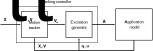
\includegraphics[]{images/trackingController}
\else
   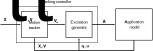
\includegraphics[width=5in]{images/trackingController}
\fi
\end{center}
\caption{Tracking controller operation for motion targets.}
\label{trackingController:fig}
\end{figure}

\subsection{Motion tracking}
\label{MotionTracking:sec}

As mentioned above, the motion tracker computes a desired source velocity
$\v_*$ for the next time step based on the current source state $(\x, \v)$ and
desired target state $(\x_t, \v_t)$. This can be done in two ways: {\it
chase control} (the default), and {\it PD control}.

\subsubsection{Chase control}
\label{ChaseControl:sec}

Chase control simply sets $\v_*$ to $\v_t$, plus an additional velocity that
tries to reduce the position error $\x_t - \x$ over a specified time interval
$T$, called the {\it chase time}:
%
\begin{equation}
\v_* = \v_t + \frac{\x_t - \x}{T}.
\label{chaseControl:eqn}
\end{equation}
%
In general, $T$ should be greater than or equal to the simulation step size
$h$. If it is greater, then $\x$ will tend to lag behind $\x_t$, but this will
also reduce the potential for overshoot due to system
nonlinearities. Conversely, if $T$ if {\it less} than $h$, then $\x$ is much
more likely to overshoot.  The default value of $T$ is 0.01.

\subsubsection{PD control}
\label{PDControl:sec}

PD control computes a desired source {\it acceleration} $\dot\v_*$ based on
%
\begin{equation}
\dot\v_* = K_p (\x_t - \x) + K_d (\v_t - \v),
\label{PDcontrol:eqn}
\end{equation}
%
and then integrates this to determine $\v_*$:
%
\begin{equation}
\v_* = \v + h \dot\v_*,
\label{PDcontrolVtarg:eqn}
\end{equation}
%
where $h$ is the simulation step size. PD control offers a greater ability to
adjust the tracking behavior than chase control, but it is often necessary to
tune the gain parameters $K_p$ and $K_d$. One rule of thumb is to
set their initial values such that (\ref{chaseControl:eqn}) and
(\ref{PDcontrolVtarg:eqn}) are equal, which leads to
%
\begin{equation*}
K_p = \frac{1}{h T}, \quad K_d = \frac{1}{h}.
\end{equation*}
%
The default values for $K_p$ and $K_d$ are $10000$ and $100$, corresponding to
$h$ and $T$ both equaling $0.01$. Lowering the value of $K_p$ will reduce
overshoot but increase tracking lag.

PD control is enabled and adjusted by setting the {\sf usePDControl}, {\sf Kp}
and {\sf Kd} properties of the motion target term to {\tt true}
(Section \ref{MotionTermProperties:sec}).

\subsection{Generating excitations using a quadratic program}
\label{GeneratingExcitations:sec}

Given $\v_*$, the excitation generator computes $\a$ to try and ensure that the
velocity at the end of the subsequent time step, $\v^{k+1}$, satisfies
%
\begin{equation}
\v^{k+1} \approx \v_*.
\label{vtrack:eqn}
\end{equation}
%
This is accomplished using a quadratic program.

First, for a broad class of problems, $\f$ is linearly related to $\a$,
so that (\ref{fnonlinear:eqn}) simplifies to
%
\begin{equation}
\f = \f_p (\q, \u) + \Lambda (\q, \u) \a,
\label{flinearInA:eqn}	
\end{equation}
where $\Lambda$ is an excitation response matrix. Given (\ref{flinearInA:eqn}),
it is possible to show (section ``Inverse modeling''
in \cite{lloyd2012artisynth}) that
%
\begin{equation*}
\v^{k+1} = \v_0 + \H_m \a,
\end{equation*}
%
where $\v_0$ is the velocity with zero excitations and $\H_m$ is a
motion excitation response matrix. To best follow the trajectory, we
can compute $\a$ to minimize the quadratic cost function
%
\begin{equation}
\phi_m(\a) \equiv \frac{1}{2} \| \v_* - \v^{k+1} \| = 
\frac{1}{2} \| \bar\v - \H_m \a \|^2, \quad
\bar\v \equiv \v_* - \v_0.
\label{MotionCostTerm:eqn}
\end{equation}
%
If we add in the constraint that excitations lie in the range $[0,
1]$, the problem takes the form of a quadratic program (QP)
%
\begin{gather}
\min_{\a} \; \phi_m(\a) \notag \\
\text{subject to} \quad 0 \le \a \le {\bf 1}.
\label{basicQP:eqn}
\end{gather}
%
In order to prioritize some target terms over others,
$\phi_m(\a)$ can be modified to include weights, according to
%
\begin{equation}
\phi_m(\a) \equiv \frac{1}{2} \| \W_m (\bar\v - \H_m \a) \|^2,
\label{motionCostTerm:eqn}	
\end{equation}
%
where $\W_m$ is a diagonal weighting matrix.
%
To handle excitation redundancy, where the size of $\a$ exceeds the
size of $\v$, we can add a regularization term
$\frac{1}{2} \a^T \W_a \a$, where $\W_a$ is a diagonal weight matrix that
can be used to adjust the relative importance of specific excitations:
%
\begin{gather}
\min_{\a} \; \phi_m(\a) + \frac{1}{2} \a^T \W_a \a \notag \notag \\
\text{subject to} \quad 0 \le \a \le {\bf 1}.
\label{regularizedQP:eqn}
\end{gather}
%

\begin{sideblock}
The matrix $\W_a$ described here is the {\it inverse} of the matrix $\W$
presented in \cite{lloyd2012artisynth}.
\end{sideblock}

\subsection{Force tracking}
\label{ForceTracking:sec}

Other cost terms can be added to the tracking controller.  For
instance, we can request a force trajectory $\f_{et}$ for a selected set
of force effectors. As with motions, the forces of these effectors
$\f_e$ at the end of step $k+1$ are linearly related to $\a$ via
%
\begin{equation*}
\f_e^{k+1} = \f_{e0} + \H_e \a
\end{equation*}
%
where $\f_{t0}$ is the force with zero excitations and $\H_e$ is
the force excitation response matrix. The force trajectory can
then be tracking by minimizing
%
\begin{equation}
\phi_e(\a) \equiv \frac{1}{2} \| \W_e (\bar\f_e - \H_e \a) \|^2, \quad
\bar\f_e \equiv \f_{et} - \f_{e0},
\label{forceEffectorCostTerm:eqn}	
\end{equation}
%
where $\W_e$ is a diagonal weighting matrix.
%ikewise, we can request a trajectory $\f_{c*}$ for selected
%constraint forces $\f_c$ in the bilateral contraints (e.g., joints),
%by minimizing
%%
%\begin{equation}
%\phi_c(\a) \equiv \frac{1}{2} \| \W_c (\bar\f_c - \H_c \a) \|^2, \quad
%\bar\f_c \equiv \f_{c*} - \f_{c0}.
%\label{constraintForceCostTerm:eqn}	
%\end{equation}
%%
%where $\W_c$ is again a diagonal weighting matrix.
When tracking force targets, the target force trajectory $\f_{et}$ is fed
directly into the excitation generator (Figure \ref{trackingForces:fig}); there
is no equivalent of the motion tracker.

\begin{figure}[ht]
\begin{center}
\iflatexml
   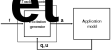
\includegraphics[]{images/trackingForces}
\else
   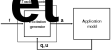
\includegraphics[width=3.5in]{images/trackingForces}
\fi
\end{center}
\caption{Tracking controller operation for force targets.}
\label{trackingForces:fig}
\end{figure}

To balance the effect of different cost terms, each is associated with
a weight (e.g., $w_m$, $w_e$, and $w_a$ for the motion, force and
regularization terms), so that the QP takes a form such as
%
\begin{gather}
\min_{\a} \; w_m \phi_m(\a) + w_e \phi_f (\a) + \frac{w_a}{2} \a^T \W_a \a \notag \\
\text{subject to} \quad 0 \le \a \le {\bf 1}.
\label{fullQP:eqn}
\end{gather}
%

\subsection{Incremental computation}
\label{IncrementalComputation:sec}

In some cases, the system forces are {\it not} linear with respect to the
excitations (i.e., equation (\ref{flinearInA:eqn}) is not valid). One
situation where this occurs is when equilibrium muscle models are used
(Section \ref{equilibriumMuscles:sec}).

When forces are not linear in $\a$, the force relationship can be linearized
and the quadratic program can be reformulated in terms of excitation {\it
changes} $\Delta \a$; for example,
%
\begin{gather}
\min_{\Delta\a} \; w_m \phi_m(\Delta\a) + w_e \phi_f (\Delta\a) + 
\frac{w_a}{2} \Delta\a^T \W_a \Delta\a + \a_0^T \W_a \Delta\a \notag \\
\text{subject to} \quad -\a_0 \le \Delta\a \le {\bf 1-\a_0}.
\label{incrementalQP:eqn}
\end{gather}
%
where $\a_0$ denotes the excitation values at the beginning of
the time step. Excitations are then updated
according to 
%
\begin{equation*}
\a = \a_0 + \Delta \a.
\end{equation*}
%

Incremental computation can be enabled, at the expense of slower computation,
by setting the tracking controller property {\sf computeIncrementally} to {\tt
true} (Section \ref{ControllerProperties:sec}).

\subsection{Setting up the tracking controller}
\label{SettingUpController:sec}

Applications will generally set up a tracking controller using the following
steps inside the application's {\tt build()} method:

\begin{enumerate}

\item Create an instance of 
\javaclass[\inverse]{TrackingController} and add it to the application
using the root model's
\javamethod[artisynth.core.workspace.RootModel]{addController()} method.

\item Configure the controller with the available excitation components 
using its
\javamethodAlt{\inverse.TrackingController.addExciter()}{addExciter(ex)}
and
\javamethodAlt{\inverse.TrackingController.addExciter(,)}{addExciter(weight,ex)}
methods.

\item Configure the controller to track position or force
trajectories for selected source components, which may include
\javaclass[\mech]{Point},
\javaclass[\mech]{Frame},
or 
\javaclass[\mech]{ForceEffector}
components. These are specified to the controller using methods such as
\javamethodAlt{\inverse.TrackingController.addPointTarget()}%
{addPointTarget(point)},
\javamethodAlt{\inverse.TrackingController.addFrameTarget()}%
{addFrameTarget(frame)},
and 
\javamethodAlt{\inverse.TrackingController.addForceEffectorTarget()}%
{addForceEffectorTarget(forceEffector)}. These methods return a {\it target}
object, which is allocated and maintained by the controller, and which is used
for specifying the target positions or forces.

\item Create input probes or controllers to specify the desired
trajectories for the sources added in Step 3. Trajectories are specified by
using probes or controllers to set the appropriate target properties of the
target objects returned by the {\tt addXXXTarget()} methods.  Likewise, output
probes or monitors can be created to record the excitations and the tracked
positions or forces of the sources.

\item Add other cost terms as needed. These may include
an L2 regularization term, added using the controller's
\javamethodAlt{\inverse.TrackingController.addL2RegularizationTerm()}%
{addL2RegularizationTerm()} method. Regularization attempts to minimize the norm
of the excitation values and is needed to resolve redundancy if the excitation
set has more degrees of freedom that the target space.

\item Set controller configuration parameters.

\end{enumerate}

Once the tracking controller has been set up, during subsequent simulation it
will compute excitation values, using the quadratic program described in
Sections \ref{GeneratingExcitations:sec} and \ref{ForceTracking:sec}, so as to
best follow the prescribed target trajectories.

\subsection{Example: moving a point with multiple Muscles}
\label{InverseParticle:sec}

\begin{figure}[ht]
\begin{center}
\begin{tabular}{cc}
   \iflatexml
      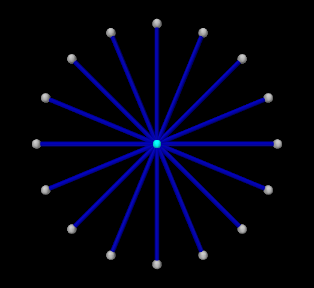
\includegraphics[]{images/InverseParticleA}&
      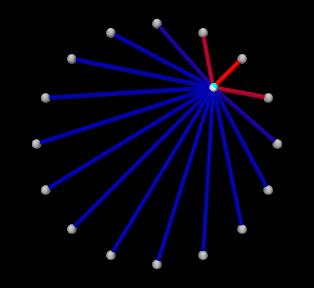
\includegraphics[]{images/InverseParticleB}
   \else
      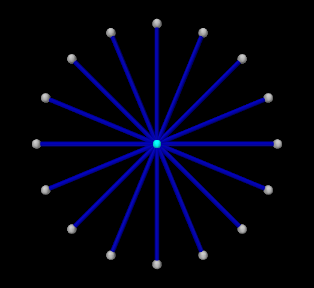
\includegraphics[width=3in]{images/InverseParticleA}&
      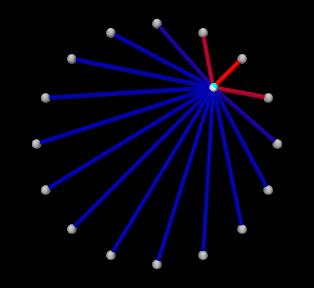
\includegraphics[width=3in]{images/InverseParticleB}
   \fi
\end{tabular}
\end{center}
\caption{{\tt InverseParticle} when first loaded (left), and
during simulation with the muscles activated to move
the center particle (right).}
\label{InverseParticle:fig}
\end{figure}

\begin{figure}[ht]
\begin{center}
\iflatexml
   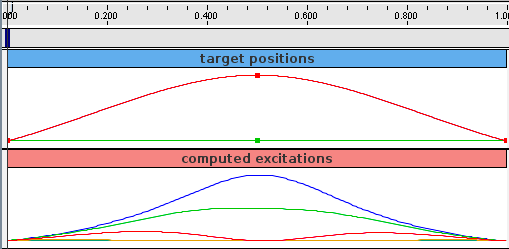
\includegraphics[]{images/InverseParticleProbes}
\else
   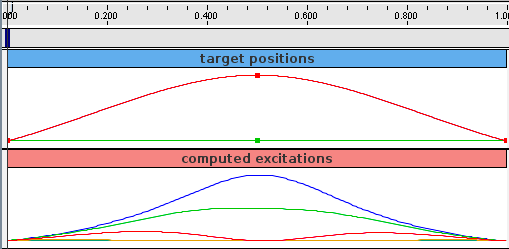
\includegraphics[width=4in]{images/InverseParticleProbes}
\fi
\end{center}
\caption{Probes showing the target position and computed
excitations for {\tt InverseParticle}.}
\label{InverseParticleProbes:fig}
\end{figure}

An simple example illustrating the steps of
Section \ref{SettingUpController:sec} is given by
%
\begin{verbatim}
  artisynth.demos.tutorial.InverseParticle
\end{verbatim}
%
which uses a set of point-to-point muscles to drive the position of a single
particle. The model consists of a single dynamic particle, initially located at
the origin, attached to a set of 16 point-to-point muscles arranged radially
around it. A tracking controller is created to control the excitations of these
muscles so as to enable the particle to follow a trajectory specified by a
probe. The code for the model, without the package and include directives, is
listed below:
%
\lstset{numbers=left}
\iflatexml
%% Hack: latexml lstinputlisting doesn't handle firstline correctly
\lstset{firstnumber={-23}}
\lstinputlisting[firstline=1]{../../src/artisynth/demos/tutorial/InverseParticle.java}
\lstset{firstnumber={1}}
\else
\lstinputlisting[firstline=25]{../../src/artisynth/demos/tutorial/InverseParticle.java}
\fi
\lstset{numbers=none}
%

The {\tt build()} method begins by creating a {\tt MechModel} in the usual way
and disabling gravity (lines 35-37). The particle to be controlled is then
created and placed at the origin and with a damping factor of 0.1 (lines
40-42). Next, the particle is attached to a set of point-to-point muscles that
are arranged radially around it (lines 45-48). These are created using the
method {\tt createMuscle()} (lines 13-31), which attaches each to a fixed
non-dynamic particle located a distance of {\tt dist} from the origin, and sets
its material to a {\tt SimpleAxialMuscle} (Section \ref{SimpleAxialMuscle:sec})
with a passive stiffness, damping and maximum force (at excitation 1) defined
by {\tt muscleStiffness}, {\tt muscleDamping}, and {\tt muscleFmax} (lines
4-6). Each muscle's {\sf excitationColor} and {\sf maxColoredExcitation}
property is set so that its color transitions to red as its excitation value
varies from $0$ to $0.5$ (lines 28-29, Section \ref{ExcitationColoring:sec})),
and its rest length is initialized to its current length (line 30).

After the model components have been built, a {\tt TrackingController} is
created and added to the root model's controller set (lines 51-52).  All of the
muscles are then added to the controller as exciters to be controlled (lines
54-58). The particle is added to the controller as a motion source using the
{\tt addPointTarget()} method (line 60), which returns a {\tt target} object
in the form of a {\tt TargetPoint}. Since the number of exciters exceeds the
degrees-of-freedom of the target space, an L2-regularization term is added
(line 63) to resolve the redundancy.

Rendering properties are set at lines 67-69: points in the model are rendered
as gray spheres, except for the dynamic particle which is colored white, and
the muscles are drawn as blue cylinders. (The {\tt target} particle, which is
contained within the controller, is displayed using its default color of cyan.)

Probes are created to specify the target trajectory and record the computed
excitations. The first, {\tt targetprobe}, is an input probe attached to the
{\sf position} property of the {\tt target} component, running from time 0 to 1
(lines 72-79). Its data is specified in code using {\tt addData()}, which
specifies three knot points with a time step of 0.5. Interpolation is set to
cubic (line 78) for greater smoothness. The second, {\tt exprobe}, is a probe
that records all the excitations computed by the controller (lines 82-85).  It
is created by the utility method {\tt createOutputProbe()} supplied by
the \javaclass[\inverse]{InverseManager} class
(Section \ref{InverseManagerProbes:sec}).

To run this example, select {\sf All demos > tutorial > InverseParticle} from
the {\sf Models} menu. The model should load and initially appear as in
Figure \ref{InverseParticle:fig} (left). When run, the controller computes
excitations to move the particle along the trajectory specified by the probe,
which is upward and to the right (Figure \ref{InverseParticle:fig}, right) and
back again. 

The target point created by the controller is rendered separately from the
source point as a cyan-colored sphere (see
Section \ref{MotionTargetRendering:sec}). As the simulation proceeds and
certain muscles are excited, their coloring changes from blue to red, in
proportion to their excitation, in accordance with the properties {\sf
excitationColor} and {\sf maxColoredExcitation}. Recorded data for both the
trajectory and the computed excitation probes are shown in
Figure \ref{InverseParticleProbes:fig}.

\section{Tracking controller components}

This section describes in greater detail how exciters, motion and force
sources, and other cost terms can be specified for the controller.

\subsection{Exciters}
\label{Exciters:sec}

An exciter can be any model component that implements
\javaclass[\mech]{ExcitationComponent}. These include
point-to-point {\tt Muscles} (Section \ref{PointToPointMuscles:sec}), muscle
bundles in FEM muscle models (Section \ref{MuscleBundles:sec}), and {\tt
MuscleExciter}s (Section \ref{MuscleExciters:sec}). Each exciter exports an
{\sf excitation} property which accepts a scalar input signal (usually in the
range $[0,1]$) that drives the exciter's active force (or fans it out to other
exciters in the case of a {\tt MuscleExciter}).

The set of excitation components used by a tracking controller is managed by
the following methods:

%
\begin{methodtable}{0.58}{0.42}
\midline
%
\methodentry
{\inverse.TrackingController.addExciter(ExcitationComponent)}%
{void addExciter(ExcitationComponent ex)}%
{Adds an exciter with default weight 1.0.}%
%
\methodentry
{\inverse.TrackingController.addExciter(double,ExcitationComponent)}%
{void addExciter(double w, ExcitationComponent ex)}%
{Adds an exciter with weight {\tt w}.}%
%
\methodentry
{\inverse.TrackingController.addExciters(Collection)}%
{void addExciters(Collection<ExcitationComponent> exciter)}%
{Adds a collection of exciters with weights 1.0.}%
%
\methodentry
{\inverse.TrackingController.numExciters()}%
{int numExciters()}%
{Returns the number of exciters.}%
%
\methodentry
{\inverse.TrackingController.getExciter(int)}%
{ExcitationComponent getExciter (int idx)}%
{Returns the idx-th exciter.}%
%
\methodentry
{\inverse.TrackingController.getExciters()}%
{ListView<ExcitationComponent> getExciters()}%
{Returns a list of all exciters.}%
%
\methodentry
{\inverse.TrackingController.clearExciters()}%
{void clearExciters()}%
{Remove all exciters.}%
%
\midline
\end{methodtable}
%

An exciter's weight forms its corresponding entry in the diagonal matrix $\W_a$
used by the quadratic program ((\ref{regularizedQP:eqn} and
(\ref{fullQP:eqn})), with a smaller weight allowing the exciter to assume
greater prominence in the solution.

By default, the computed excitations are bounded by the interval $[0,1]$, as
indicated in Section \ref{GeneratingExcitations:sec}. However, these bounds can
be altered, either collectively using the tracking controller property {\sf
excitationBounds}, or individually for specific exciters:

%
\begin{methodtable}{0.58}{0.42}
\midline
%
\methodentry
{\inverse.TrackingController.setExcitationBounds(DoubleInterval)}%
{void setExcitationBounds(DoubleInterval range)}%
{Sets the excitationBounds property.}%
%
\methodentry
{\inverse.TrackingController.getExcitationBounds()}%
{DoubleInterval getExcitationBounds()}%
{Queries the excitationBounds property.}%
%
\methodspace{0.5em}%
%
\methodentry
{\inverse.TrackingController.setExcitationBounds(ExcitationComponent,,)}%
{void setExcitationBounds(ExcitationComponent ex,\brh double low, double high)}%
{Sets excitation bounds for exciter {\tt ex}.}%
%
\methodentry
{\inverse.TrackingController.getExcitationBounds(ExcitationComponent)}%
{DoubleInterval getExcitationBounds(ExcitationComponent ex)}%
{Queries excitation bounds for exciter {\tt ex}.}%
%
\midline
\end{methodtable}
%

The excitation values themselves can also be queried and set with the following
methods:
%
\begin{methodtable}{0.58}{0.42}
\midline
%
\methodentry
{\inverse.TrackingController.getExcitations(VectorNd)}%
{void getExcitations(VectorNd values)}%
{Returns excitations in {\tt values}.}%
%
\methodentry
{\inverse.TrackingController.getExcitation(int)}%
{double getExcitation(int idx)}%
{Returns the excitation of the idx-th exciter.}%
%
\midline
\end{methodtable}
%

By default, the controller initializes excitations to zero and then updates
them at the beginning of each time step. However, when excitations are being
computed incrementally (Section \ref{IncrementalComputation:sec}), it may be
desirable to start with non-zero excitation values. In that case, the following
methods may be useful:
%
\begin{methodtable}{0.58}{0.42}
\midline
%
\methodentry
{\inverse.TrackingController.initializeExcitations()}%
{void initializeExcitations()}%
{Sets excitations to the current exciter values.}%
%
\methodentry
{\inverse.TrackingController.setExcitations(VectorNd)}%
{void setExcitations(VectorNd values)}%
{Sets excitations to {\tt values}.}%
%
\midline
\end{methodtable}
%
The first sets the controller's internal excitation values to those stored in
the exciters, while the second sets both the internal values and the values in
the exciters.

\subsubsection{Excitation coloring}
\label{ExcitationColoring:sec}

Some exciters (such as {\tt Muscle} and {\tt MultiPointMuscle}) support the
ability to change color in proportion to their excitation value. This makes it
easier to visualize the extent to which exciters are being activated within the
model. Exciters which support this capability export the properties {\sf
excitationColor}, which is the color the exciter should transition to as
excitation is increased, and {\sf maxColoredExcitation}, which the excitation
value at which the color transition is complete.  In other words, the exciter's
color will vary from its default color to {\sf excitationColor} as its excitation
varies from 0 to {\sf maxColoredExcitation}.

Excitation coloring does not occur if the exciter's {\sf excitationColor} is
set to {\tt null}.

The tracking controller exports a property, {\tt configExcitationColoring},
which if true enables the automatic configuration of excitation coloring for
exciters that support this capability. If enabled, then as these exciters are
added to the controller, their {\sf excitationColor} is inspected.  If it has
not been set (i.e., if it is {\tt null}), then it is set to red and the nominal
color for the exciter is set to white, enabling a white-to-red color transition
for the exciter as it is activated.

\subsection{Motion targets}

As indicated above, motion source components can be specified to the controller
using the {\tt addPointTarget()} and {\tt addFrameTarget()} methods. Source
components may be instances of \javaclass[\mech]{Point}
or \javaclass[\mech]{Frame}, and thereby may include both FEM nodes and rigid
bodies. The methods for managing motion targets include:
%
\begin{methodtable}{0.58}{0.42}
\midline
%
\methodentry
{\inverse.TrackingController.addPointTarget(Point)}%
{TargetPoint addPointTarget(Point source)}%
{Adds point {\tt source} with weight 1.0.}%
%
\methodentry
{\inverse.TrackingController.addPointTarget(Point,double)}%
{TargetPoint addPointTarget(Point source, double w)}%
{Adds point {\tt source} with weight {\tt w}.}%
%
\methodentry
{\inverse.TrackingController.addFrameTarget(Frame)}%
{TargetFrame addFrameTarget(Frame source)}%
{Adds frame {\tt source} with weight 1.0.}%
%
\methodentry
{\inverse.TrackingController.addFrameTarget(Frame,double)}%
{TargetFrame addFrameTarget(Frame source, double w)}%
{Adds frame {\tt source} with weight {\tt w}.}%
%
\methodspace{0.5em}
%
\methodentry
{\inverse.TrackingController.numMotionTargets()}%
{int numMotionTargets()}%
{Number of motion targets.}%
%
\methodentry
{\inverse.TrackingController.removeMotionTarget(MotionTargetComponent)}%
{void removeMotionTarget(MotionTargetComponent source)}%
{Removes motion source.}%
%
\midline
\end{methodtable}
%

The {\tt addPointTarget()} and {\tt addFrameTarget()} methods each create and
return a {\it target} component, allocated and contained within the controller,
that mirrors the type of source component.  These target components are
either \javaclass[\inverse]{TargetPoint} for point sources or
\javaclass[\inverse]{TargetFrame} for frame sources.
Both {\tt TargetPoint} and {\tt TargetFrame}, together with the source
components {\tt Point} and {\tt Frame}, are instances of
\javaclass[\mech]{MotionTargetComponent}.

As simulation proceeds, the desired trajectory position $\x_t$ for each
source component is specified by setting the target component's {\sf position}
property (or {\sf position}, {\sf orientation} and/or {\sf pose} properties for
frame targets).  As described elsewhere, this can be done using either probes
or other controller objects.

Likewise, a corresponding velocity trajectory $\v_t$ can also be specified by
setting the {\sf velocity} property of the target object.  If this is not set,
$\v_t$ defaults to 0, which will introduce a small lag into the tracking
behavior. If $\v_t$ {\it is} set, care should be taken the ensure that it is
consistent with the actual time derivative of $\x_t$.

\begin{sideblock}
Applications typically do not need to specify $\v_t$. However, doing so may
improve tracking performance, particularly when using PD control
(Section \ref{MotionTracking:sec}).
\end{sideblock}

Each target component also implements the interface
\javaclass[\inverse]{TrackingTarget}, described in
Section \ref{TargetComponents:sec}, which supplies methods to specify the
weights in the weighting matrix $\W_m$ of the motion tracking cost term
$\phi_m(\a)$ (\ref{motionCostTerm:eqn}).

Lists of all the motion source components and their associated target
components (i.e., those returned by the {\tt addXXXTarget()} methods) can be
obtained using
%
\begin{methodtable}{0.58}{0.42}
\midline
%
\methodentry
{\inverse.TrackingController.getMotionSources()}%
{ArrayList<MotionTargetComponent> getMotionSources()}%
{Returns motion source components.}%
%
\methodentry
{\inverse.TrackingController.getMotionTargets()}%
{ArrayList<MotionTargetComponent> getMotionTargets()}%
{Returns motion target components.}%
%
\midline
\end{methodtable}
%

\subsubsection{Motion target term}
\label{MotionTargetTerm:sec}

The cost term $\phi_m(\a)$ that is responsible for tracking motion targets is
contained within a tracking controller subcomponent that is named {\tt
"motionTerm"} and which is an instance of
\javaclass[\inverse]{MotionTargetTerm}. Users 
may access this component directly using
%
\begin{methodtable}{0.58}{0.42}
\midline
%
\methodentry
{\inverse.TrackingController.getMotionTargetTerm()}%
{MotionTargetTerm getMotionTargetTerm()}%
{Returns the controller's motion target term.}%
%
\midline
\end{methodtable}
%
and then use it to set motion tracking properties such as those described in
Section \ref{MotionTermProperties:sec}.

The motion tracking weight $w_m$ in (\ref{fullQP:eqn}) is
given by the {\sf weight} property of the motion target term,
which can also be accessed directly by the controller methods
%
\begin{methodtable}{0.58}{0.42}
\midline
%
\methodentry
{\inverse.TrackingController.getMotionTargetTermWeight()}%}%
{double getMotionTargetTermWeight()}%
{Returns the motion target term weight.}%
%
\methodentry
{\inverse.TrackingController.setMotionTargetTermWeight()}%}%
{void setMotionTargetTermWeight(double w)}%
{Sets the motion target term weight.}%
%
%\methodspace{0.5em}%
\midline
\end{methodtable}
%

\subsubsection{Motion target rendering}
\label{MotionTargetRendering:sec}

The motion target components, which are allocated and maintained by the
controller, are rendered by default, which makes it easy to visualize
significant errors between the target positions and the tracked source
positions. Target points are drawn as cyan colored spheres.  For target frames,
if the source component corresponds to a {\tt RigidBody}, the target is
rendered using a cyan colored wireframe copy of the source's surface mesh.

Rendering of targets can be enabled or disabled by setting the tracking
controller's {\sf targetsVisible} property. Otherwise, the application is free
to set the render properties of individual target components, or their
containing lists within the {\tt MotionTargetTerm}, which can
be accessed by the methods
%
\begin{methodtable}{0.58}{0.42}
\midline
%
\methodentry
{\inverse.MotionTargetTerm.getTargetPoints()}%}%
{PointList<TargetPoint> getTargetPoints()}%
{Return all point motion target components.}%
%
\methodentry
{\inverse.MotionTargetTerm.getTargetFrames()}%}%
{RenderableComponentList<TargetFrame> getTargetFrames()}%
{Return all frame motion target components.}%
%
%\methodspace{0.5em}%
\midline
\end{methodtable}
%

Other methods of {\tt MotionTargetTerm} allow the render properties for both
the point and frame target lists to be set together:
%
\begin{methodtable}{0.55}{0.45}
\midline
%
\methodentry
{\inverse.MotionTargetTerm.getTargetRenderProps()}%
{RenderProps getTargetRenderProps()}%
{Return render properties for the motion target lists.}%
%
\methodentry
{\inverse.MotionTargetTerm.setTargetRenderProps()}%
{void setTargetRenderProps (RenderProps props)}%
{Set render properties for the motion target lists.}%
%
\methodentry
{\inverse.MotionTargetTerm.setTargetsPointRadius(double)}%
{void setTargetsPointRadius (double rad)}%
{Set {\sf pointRadius} target render property to {\tt rad}.}%
%
%\methodspace{0.5em}%
%\brh
\midline
\end{methodtable}
%

\subsection{Regularization}
\label{Regularization:sec}

\subsubsection{L2 Regularization}
\label{L2Regularization:sec}

L2 regularization attempts to minimize the weighted square of the excitation
values, as described by
%
\begin{equation}
\frac{w_a}{2} \, \a^T \W_a \, \a
\label{L2regularization:eqn}
\end{equation}
%
in (\ref{fullQP:eqn}), and so provides a way to resolve redundancy when the
number of exciters is greater than needed to perform the required tracking. It
can be enabled or disabled by adding or removing an L2 regularization term from
the controller, as managed by the following methods:
%
\begin{methodtable}{0.58}{0.42}
\midline
%
\methodentry
{\inverse.TrackingController.setL2Regularization()}%
{void setL2Regularization()}%
{Enables L2 regularization with default weight 0.0001.}%
%
\methodentry
{\inverse.TrackingController.setL2Regularization(double)}%
{void setL2Regularization(double w)}%
{Enables L2 regularization with weight {\tt w}.}%
%
\methodentry
{\inverse.TrackingController.getL2RegularizationWeight()}%
{double getL2RegularizationWeight()}%
{Returns regularization weight, or 0 if not enabled.}%
%
\methodentry
{\inverse.TrackingController.removeL2Regularization()}%
{boolean removeL2Regularization()}%
{Removes L2 regularization.}%
%
\midline
\end{methodtable}
%
The weight associated with the above methods corresponds to $w_a$ in
(\ref{L2regularization:eqn}) and (\ref{fullQP:eqn}). The entries in the
diagonal matrix $\W_a$ are given by the weights associated with the exciters
themselves, as described in Section \ref{Exciters:sec}.

L2 regularization is implemented using a controller subcomponent of type
\javaclass[\inverse]{L2RegularizationTerm}, which
is added or removed from the controller as required and can be accessed using
%
\begin{methodtable}{0.58}{0.42}
\midline
%
\methodentry
{\inverse.TrackingController.getL2RegularizationTerm()}%
{L2RegularizationTerm getL2RegularizationTerm()}%
{Returns the controller's L2 regularization term
}%
%
\midline
\end{methodtable}
%
which will return {\tt null} if regularization is not being applied.

Because the L2 regularizer tries to reduce the excitations $\a$, its use will
reduce the controller's tracking accuracy. Therefore, the regularizer is often
employed with a weight value $w_a$ well below 1.0, with values around 0.1 or
0.01 being common. The best weight choice will of coarse depend on the
application.

\subsubsection{Excitation damping}
\label{ExcitationDamping:sec}

The controller also provides a damping term that serves to minimize the time
derivative of $\a$, or more precisely,
%
\begin{equation*}
\frac{1}{2} \dot\a^T \W_a \dot\a,
\end{equation*}
%
where $\W_a$ is the diagonal excitation weight matrix used for L2
regularization (\ref{L2regularization:eqn}). Letting $\a_0$ denote
the excitations at the beginning of the time step, and approximating
$\dot\a$ by
%
\begin{equation*}
\dot\a \approx \frac{\a - \a_0}{h},
\end{equation*}
%
where $h$ is the time step size, the damping cost term $\phi_d(\a)$
becomes
%
\begin{equation*}
\phi_d(\a) = \frac{1}{2 h^2} \left( \a^T \W_a \a - 2 \a_0^T \W_a \a \right).
\end{equation*}
%
Excitation damping can be managed by the following methods:
%
\begin{methodtable}{0.6}{0.4}
\midline
%
\methodentry
{\inverse.TrackingController.setExcitationDamping()}%
{void setExcitationDamping()}%
{Enable excitation damping with default weight $10^{-5}$.}%
%
\methodentry
{\inverse.TrackingController.setExcitationDamping(double)}%
{void setExcitationDamping(double w)}%
{Enable excitation damping with weight {\tt w}.}%
%
\methodentry
{\inverse.TrackingController.getExcitationDampingWeight()}%
{double getExcitationDampingWeight()}%
{Returns damping weight, or 0 if not enabled.}%
%
\methodentry
{\inverse.TrackingController.removeExcitationDamping()}%
{void removeExcitationDamping()}%
{Removes excitation damping.}%
%
\midline
\end{methodtable}
%
Excitation damping is implemented using a controller subcomponent of type
\javaclass[\inverse]{DampingTerm}, which
is added or removed from the controller as required and can be accessed using
%
\begin{methodtable}{0.6}{0.4}
\midline
%
\methodentry
{\inverse.TrackingController.getDampingTerm()}%
{DampingTerm getDampingTerm()}%
{Returns the controller's excitation damping.}%
%
\midline
\end{methodtable}
%
which will return {\tt null} if damping is not being applied.

\subsection{Example: controlling ToyMuscleArm}
\label{InverseMuscleArm:sec}

\begin{figure}[ht]
\begin{center}
   \iflatexml
      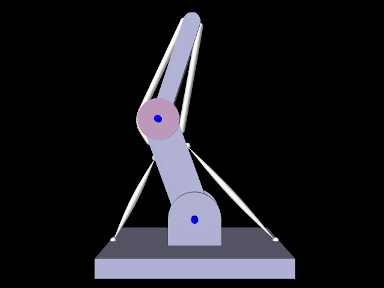
\includegraphics[]{images/InverseMuscleArm}
   \else
      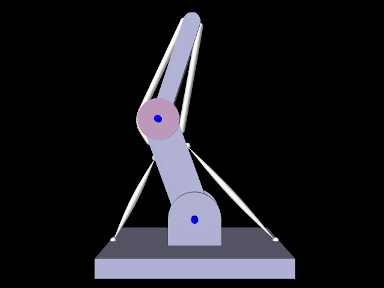
\includegraphics[width=3.75in]{images/InverseMuscleArm}
   \fi
\end{center}
\caption{{\tt InverseMuscleArm} when first loaded into ArtiSynth.}
\label{InverseMuscleArm:fig}
\end{figure}

A good tracking controller example is given by the model {\tt
artisynth.demos.tutorial.InverseMuscleArm}, which computes the muscle
excitations needed to make the tip marker of the {\tt ToyMuscleArm} demo
(described in Section \ref{ToyMuscleArm:sec}) follow a prescribed trajectory.
The model extends {\tt artisynth.demos.tutorial.ToyMuscleArm}, and then adds
the tracking controller and probes needed to move the tip marker,
as shown in the code below:
%
\lstset{numbers=left}
\iflatexml
%% Hack: latexml lstinputlisting doesn't handle firstline correctly
\lstset{firstnumber={-25}}
\lstinputlisting[firstline=1]{../../src/artisynth/demos/tutorial/InverseMuscleArm.java}
\lstset{firstnumber={1}}
\else
\lstinputlisting[firstline=27]{../../src/artisynth/demos/tutorial/InverseMuscleArm.java}
\fi
\lstset{numbers=none}
%

As mentioned above, this model extends {\tt ToyMuscleArm} (line 1), and so
calls {\tt super.build(args)} in the {\tt build()} method to create all the
components of {\tt ToyMuscleArm}. Once this is done, the link positions are
adjusted by setting the hinge joint angles (lines 8-9); this is done to move
the arm away from the kinematic singularity at full extension and thus make it
easier for the tip to follow a prescribed path. After the links are moved, the
all wrap paths are updated by calling the {\tt MechModel} method {\tt
updateWrapPath()} (line 10).

A tracking controller is then created (lines 13-14), and every {\tt
Muscle} and {\tt MultiPointMuscle} is added to it as an exciter (lines 17-24).
When iterating through the muscles, their rest lengths are reinitialized to
their current lengths (which changed when the links were repositioned) to
ensure that passive muscle forces are zero in the initial position.

Next, the marker at the tip of link1 (referenced by the inherited attribute
{\tt myTipMkr}) is added to the controller as a motion source (line 27) and
the returned target object is stored in {\tt target}.  An L2 regularization
term is added to the controller with weight 0.01 (line 29), and an input probe
is created to provide the marker trajectory by setting the target's {\tt
position} property (lines 31-46). The probe has a duration of 5 seconds, and
the trajectory is a closed path, specified by 5 cubically interpolated knot
points (line 43), that lie in the x-z plane and start at and return to the
marker's initial position {\tt x0}, {\tt z0}.

Probes are created to record the computed excitations and trace the
desired and actual trajectories in the viewer. The first, {\tt
exprobe}, is created by the utility method {\tt
createOutputProbe()} supplied by the
\javaclass[\inverse]{InverseManager} class 
(lines 49-52, Section \ref{InverseManagerProbes:sec}). The tracing probes
are created by the {\tt RootModel} method
\javamethod[artisynth.core.workspace.RootModel]{addTracingProbe()} (lines
56-62), and two are created: one to trace the desired target by recording the
{\sf position} property of {\tt target}, and another to trace the actual
tracked (source) position by recording the {\sf position} property of {\tt
myTipMkr}. The line colors of these are set to cyan and red, respectively,
which specifies their display color in the viewer.

Lastly, an {\it inverse control panel} (Section \ref{InverseControlPanel:sec})
is created to manage controller properties (line 65), and some settings are
made to allow for probe management by the 
\javaclass[\inverse]{InverseManager} class, as discussed
in Section \ref{InverseManagerProbes:sec} (lines 67-70); this includes setting
the default probe duration to {\tt stopTime} and the working folder to {\tt
inverseMuscleArm} located under the source folder.

\begin{figure}[ht]
\begin{center}
\begin{tabular}{cc}
   \iflatexml
      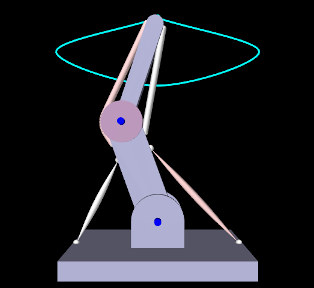
\includegraphics[width=3.25in]{images/InverseMuscleArmL2_reg}&
      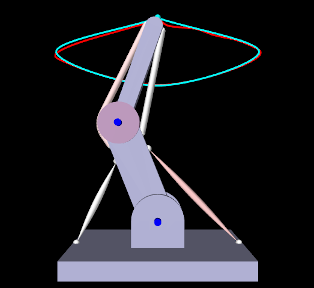
\includegraphics[width=3.25in]{images/InverseMuscleArmL2_10}\\
      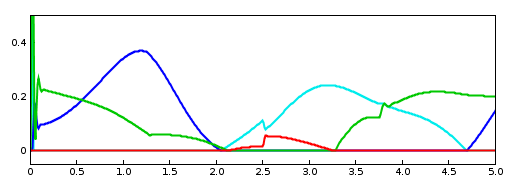
\includegraphics[width=3.25in]{images/InverseMuscleArmExL2_reg}&
      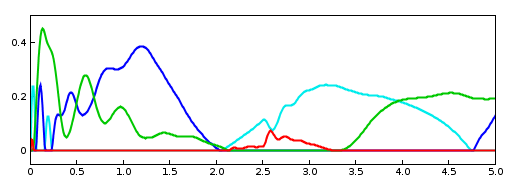
\includegraphics[width=3.25in]{images/InverseMuscleArmExL2_10}\\
   \else
      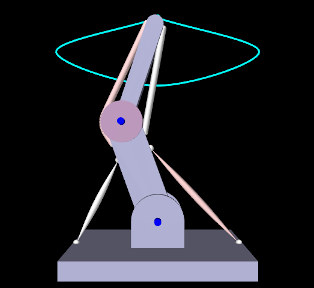
\includegraphics[width=3.25in]{images/InverseMuscleArmL2_reg}&
      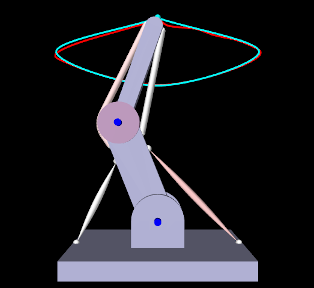
\includegraphics[width=3.23in]{images/InverseMuscleArmL2_10}\\
      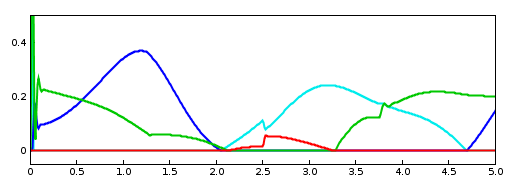
\includegraphics[width=3.25in]{images/InverseMuscleArmExL2_reg}&
      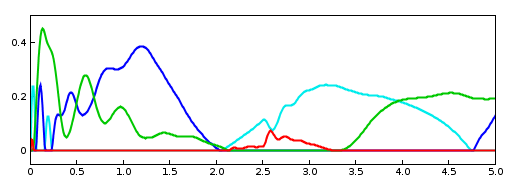
\includegraphics[width=3.23in]{images/InverseMuscleArmExL2_10}
   \fi
\end{tabular}
\end{center}
\caption{{\tt InverseMuscleArm} run with L2 regularization weights of 0.1
(left) and 10 (right). Traces of the desired and actual trajectories are shown
in cyan and red, respectively, and computed excitation values are shown in
graphs below.  A regularization weight of 10results in a larger tracking
error.}
\label{InverseMuscleArmL2:fig}
\end{figure}

To run this example, select {\sf All demos > tutorial > InverseMuscleArm} from
the {\sf Models} menu. The model should load and initially appear as in Figure
\ref{InverseMuscleArm:fig}. When run, the controller will compute excitations to
make the tip marker trace the desired trajectory, as shown in Figure
\ref{InverseMuscleArmL2:fig} (left), where the tracing probe shows the
target trajectory in cyan; the source trajectory appears beneath it in red but
is largely invisible because it follows the target quite accurately.  Computed
excitation values are shown below. The target component created for the tip
marker is rendered as a cyan-colored sphere
(Section \ref{MotionTargetRendering:sec}).

\begin{sideblock}
The muscles in {\tt InverseMuscleArm} are initially colored white instead of
red (as they are for {\tt ToyMuscleArm}). That is because if a muscle's {\sf
excitationColor} property is {\tt null}, the controller automatically
configures the muscle to vary in color from white to red as the muscle is
activated, as described in Section \ref{ExcitationColoring:sec}.  This
behavior can be disabled by setting the controller property {\sf
configExcitationColoring} to {\tt false}.
\end{sideblock}

To illustrate how the L2 regularization weight can affect the tracking error,
\ref{InverseMuscleArmL2:fig} (right) shows the model run with a regularization
weight of 10 instead of 0.1. The tracking error is now visible, with the red
source trace probe clearly distinct from the cyan target trace. The computed
muscle excitations are also noticeably different.

\subsection{Example: controlling an FEM muscle model}
\label{InverseMuscleFem:sec}

\begin{figure}[ht]
\begin{center}
\begin{tabular}{cc}
   \iflatexml
      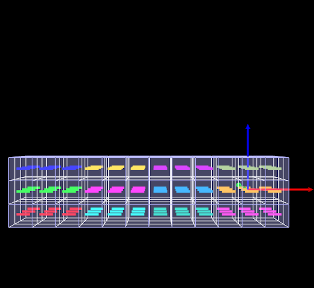
\includegraphics[]{images/InverseMuscleFemA}
      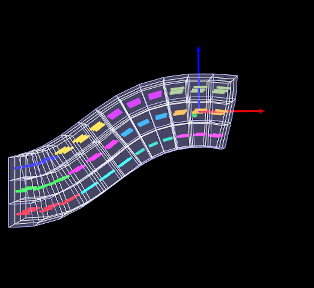
\includegraphics[]{images/InverseMuscleFemB}
   \else
      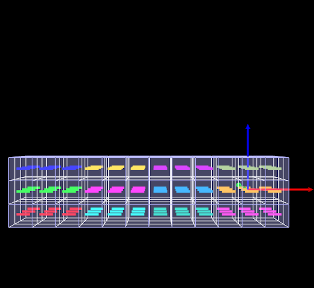
\includegraphics[width=3in]{images/InverseMuscleFemA}
      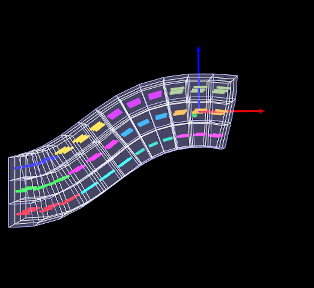
\includegraphics[width=3in]{images/InverseMuscleFemB}
   \fi
\end{tabular}
\end{center}
\caption{{\tt InverseMuscleFem} when first loaded into ArtiSynth (left),
and after executing in the inverse simulation (right).}
\label{InverseMuscleFem:fig}
\end{figure}

Another example involving an FEM muscle model is given by {\tt
artisynth.demos.tutorial.InverseMuscleFem}, which computes the muscle
excitations needed to make an attached frame of the {\tt ToyMuscleFem} demo
(described in Section \ref{ToyMuscleFem:sec}) follow a prescribed trajectory.

The model extends {\tt artisynth.demos.tutorial.ToyMuscleFem}, and then adds
the tracking controller and probes needed to move the tip marker, as shown in
the code below:
%
\lstset{numbers=left}
\iflatexml
%% Hack: latexml lstinputlisting doesn't handle firstline correctly
\lstset{firstnumber={-16}}
\lstinputlisting[firstline=1]{../../src/artisynth/demos/tutorial/InverseMuscleFem.java}
\lstset{firstnumber={1}}
\else
\lstinputlisting[firstline=18]{../../src/artisynth/demos/tutorial/InverseMuscleFem.java}
\fi
\lstset{numbers=none}
%

Since the model extends {\tt ToyMuscleFem} (line 1), the {\tt build()} method
begins by calling {\tt super.build(args)} to create the model defined by the
superclass. A tracking controller is then created and added to the root model's
controller set, all the muscle bundles in the FEM muscle model are added to it
as exciters, and the attached frame is added to it as a motion source using {\tt
addFrameTarget} (lines 9-16).

An L2 regularization term is added, and then the motion tracking is set to use
PD control (Section \ref{MotionTracking:sec}), using gains of $K_p =
1000$ and $K_d = 100$ (line 19-23).

To control position and orientation of the frame, two input probes are created
(lines 27-38), one attached to the target's {\sf position} and the other to its
{\sf orientation}.  (While it is possible to use a single probe to control both
of these properties, or the single {\sf pose} property, separate probes are
used here to provide easier visualization.) Their data and settings are read
from the probe files {\tt inverseFemFramePos.txt} and {\tt
inverseFemFrameRot.txt}, located in the folder {\tt data} beneath the
application model source folder. Each specifies a probe in the time range from
0 to 5, with 26 knot points and cubic interpolation.

\begin{figure}[h]
\begin{center}
\begin{tabular}{c}
   \iflatexml 
      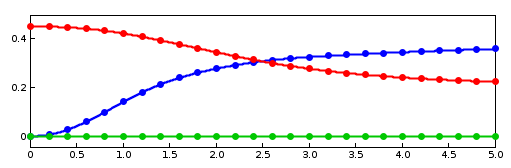
\includegraphics[]{images/InverseMuscleFemTarget}\\
      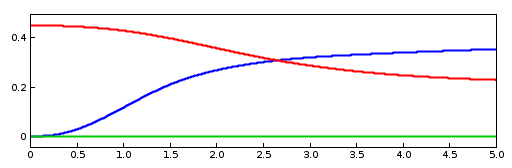
\includegraphics[]{images/InverseMuscleFemSource}\\
      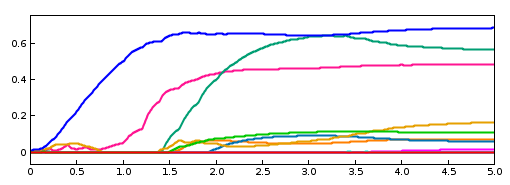
\includegraphics[]{images/InverseMuscleFemEx} 
   \else
      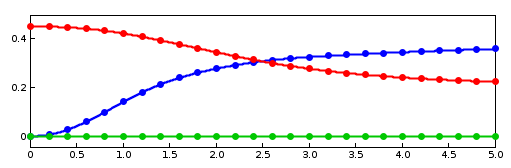
\includegraphics[width=3.25in]{images/InverseMuscleFemTarget}\\
      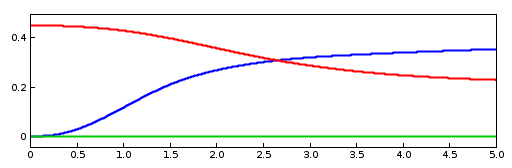
\includegraphics[width=3.25in]{images/InverseMuscleFemSource}\\
      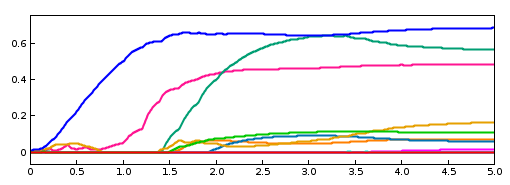
\includegraphics[width=3.25in]{images/InverseMuscleFemEx}
   \fi
\end{tabular}
\end{center}
\caption{Probe data generated by {\tt InverseMuscleFem}. Top:
target trajectory for the frame position (26 knot points, cubically
interpolated). Middle: actual position tracked by the controller.
Bottom: computed muscle excitations.}
\label{InverseMuscleFemProbes:fig}
\end{figure}

To monitor the controller's tracking performance, two output probes are created
and attached to the {\sf position} and {\sf orientation} properties of the
source component {\tt myFrame} (lines 58-67). Setting the {\tt interval}
argument to -1 in the probes' constructors causes them to use the model's
current step size as the update interval. Finally, the utility class
\javaclass[\inverse]{InverseManager} (Section \ref{InverseManager:sec}) 
is used to create an output probe for the computed excitations, as well as a
control panel giving access to the various controller properties (lines 70-75).

To run this example, select {\sf All demos > tutorial > InverseMuscleFem} from
the {\sf Models} menu. The model should load and initially appear as in Figure
\ref{InverseMuscleFem:fig} (left). When run, 
the controller will compute excitations to move the attached frame along the
specified position/orientation trajectory, reaching the final pose shown in
Figure \ref{InverseMuscleFem:fig} (right). The target and actual source
trajectories for the frame's position (i.e., its origin) is shown in Figure
\ref{InverseMuscleFemProbes:fig}, together with the computed excitations.

\subsection{Force effector targets}

The controller can also be asked to track a force trajectory for a set of force
effector components; the excitations will then be computed to try to
generate the prescribed forces. Any force component that implements the
interface \javaclass[\mech]{ForceTargetComponent} can be used as a force
effector source; this interface extends 
\javaclass[\mech]{ForceEffector} to supply several additional
methods including:
%
\begin{lstlisting}[]
interface ForceTargetComponent extends ForceEffector, ModelComponent {

   // gets the dimension of the generated force
   public int getForceSize(); 

   // returns the current force value
   public void getForce (VectorNd minf, boolean staticOnly);

   ...
}
\end{lstlisting}
%
At the time of this writing, {\tt ForceTargetComponent}s include:
%
\begin{center}
\begin{tabular}{|lcl|}
\hline
Component & Force size & Force description\\
\hline
\javaclass[\mech]{AxialSpring} & 1 & Tension in the spring\\
\javaclass[\mech]{Muscle} & 1 & Tension in the muscle\\
\javaclass[\mech]{FrameSpring} & 6 & 
Spring wrench as seen in body A (world coordinates)\\
\hline
\end{tabular}
\end{center}
%

Controller methods for adding and managing force effector targets include:
%
\begin{methodtable}{0.58}{0.42}
\midline
%
\methodentry
{\inverse.TrackingController.addForceEffectorTarget(ForceTargetComponent)}%
{ForceEffectorTarget addForceEffectorTarget (\brh ForceTargetComponent source)}%
{Adds static-only force source with weight 1.0}%
%
\methodentry
{\inverse.TrackingController.addForceEffectorTarget(ForceTargetComponent,)}%
{ForceEffectorTarget addForceEffectorTarget (\brh 
ForceTargetComponent source, double w)}%
{Adds static-only force source with weight {\tt w}.}%
%
\methodentry
{\inverse.TrackingController.addForceEffectorTarget(ForceTargetComponent,,)}%
{ForceEffectorTarget addForceEffectorTarget (\brh 
ForceTargetComponent source, double w, boolean staticOnly)}%
{Adds force source with weight {\tt w} and static-only specified.}%
%
\methodspace{0.5em}
%
\methodentry
{\inverse.TrackingController.numForceEffectorTargets()}%
{int numForceEffectorTargets()}%
{Number of force effector targets.}%
%
\methodentry
{\inverse.TrackingController.removeForceEffectorTarget(ForceTargetComponent)}%
{boolean removeForceEffectorTarget(\brh ForceTargetComponent source)}%
{Removes force source.}%
%
\midline
\end{methodtable}

The {\tt addForceEffectorTarget()} methods each create and return a
\javaclass[\inverse]{ForceEffectorTarget} component. 
As simulation proceeds, the desired target force for the source component is
specified by setting the target component's {\sf targetForce} property.  As
described elsewhere, this can be done using either probes or other controller
objects.  The target component also implements the interface
\javaclass[\inverse]{TrackingTarget}, described in
Section \ref{TargetComponents:sec}, which supplies methods to specify the
weighting matrix $\W_e$ in the force effector cost term $\phi_e(\a)$
(\ref{forceEffectorCostTerm:eqn}).

By default, force effector tracking is {\it static-only}, meaning that only
static forces (i.e., forces that are not velocity dependent, such as damping)
are considered.  However, the third {\tt addForceEffectorTarget()} method
allows this to be explicitly specified.

\iflatexml\else\clearpage\fi

Lists of all the force effector source components and their associated targets
can be obtained using the methods:
%
\begin{methodtable}{0.6}{0.4}
\midline
%
\methodentry
{\inverse.TrackingController.getForceEffectorSources()}%
{ArrayList<ForceEffectorTarget> getForceEffectorSources()}%
{Returns force effector source components.}%
%
\methodentry
{\inverse.TrackingController.getForceEffectorTargets()}%
{ArrayList<ForceEffectorTarget> getForceEffectorTargets()}%
{Returns force effector target components.}%
%
%\methodspace{0.5em}%
%\brh
\midline
\end{methodtable}
%

\begin{sideblock}
Specifying a force effector {\sf targetForce} of 0 will have the
same effect as {\it minimizing} the force associated with that force effector.
\end{sideblock}

\subsubsection{Force effector term}
\label{ForceEffectorTerm:sec}

The cost term $\phi_e(\a)$ that is responsible for tracking force effector
targets is contained within a tracking controller subcomponent named
{\tt "forceEffectorTerm"} and which is an instance of
\javaclass[\inverse]{ForceEffectorTerm}. 
This is added to the controller automatically whenever force effector tracking
is requested, and may accessed directly using
%
\begin{methodtable}{0.6}{0.4}
\midline
%
\methodentry
{\inverse.TrackingController.getForceEffectorTerm()}%
{ForceEffectorTerm getForceEffectorTerm()}%
{Returns the force effector term.}%
%
\midline
\end{methodtable}
%
The method will return {\tt null} if the force effector term is not present.

The force effector tracking weight $w_e$ in (\ref{fullQP:eqn}) is
given by the {\sf weight} property of the force effector term,
which can also be accessed directly by the controller methods
%
\begin{methodtable}{0.6}{0.4}
\midline
%
\methodentry
{\inverse.TrackingController.getForceEffectorTermWeight()}%}%
{double getForceEffectorTermWeight()}%
{Returns the force effector term weight.}%
%
\methodentry
{\inverse.TrackingController.setForceEffectorTermWeight()}%}%
{void setForceEffectorTermWeight(double w)}%
{Sets the force effector term weight.}%
%
%\methodspace{0.5em}%
\midline
\end{methodtable}
%

\subsection{Example: controlling tension in a spring}

\begin{figure}[ht]
\begin{center}
\begin{tabular}{cc}
   \iflatexml
      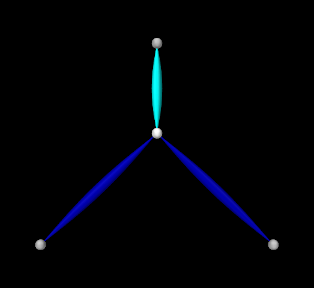
\includegraphics[]{images/InverseSpringForceA}&
      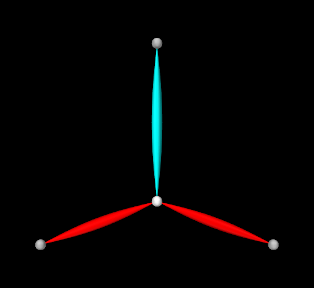
\includegraphics[]{images/InverseSpringForceB}
   \else
      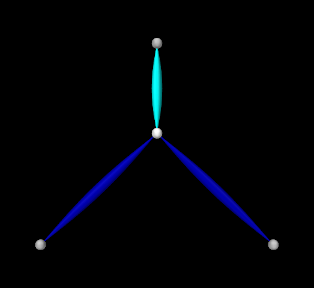
\includegraphics[width=3in]{images/InverseSpringForceA}&
      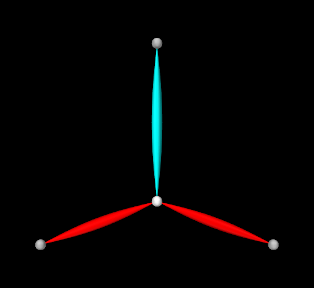
\includegraphics[width=3in]{images/InverseSpringForceB}
   \fi
\end{tabular}
\end{center}
\caption{{\tt InverseSpringForce} when first loaded (left), and
during simulation with the lower muscles fully activated to 
control the tension in the upper passive spring (cyan).}
\label{InverseSpringForce:fig}
\end{figure}

A simple example of force effector tracking is given by
%
\begin{verbatim}
  artisynth.demos.tutorial.InverseSpringForce
\end{verbatim}
%
which uses two point-to-point muscles to control the tension in a passive
spring. The initial part of the code is the same as that for {\tt
InverseParticle} (Section \ref{InverseParticle:sec}), except for different
parameter definitions,
%
\begin{lstlisting}[]
   int numMuscles = 3; // num radial muscles surrounding the dynamic particle
   double muscleStiffness = 200; // passive muscle stiffness
   double muscleDamping = 0.1; // passive muscle damping
   double muscleFmax = 200; // max active force at excitation = 1   
   double dist = 1.0; // distance of anchor point from world origin
\end{lstlisting}
%
which give the muscles different strengths and cause only 3 to be created
instead of 16, and the fact that the {\tt "center"} particle is initially placed
at $(0, 0, 0.33)$ instead of the origin. The rest of the code diverges after
the tracking controller is created, as shown below:
%
\lstset{numbers=left}
\iflatexml
%% Hack: latexml lstinputlisting doesn't handle firstline correctly
\lstset{firstnumber={-57}}
\lstinputlisting[firstline=17,lastline=67]{../../src/artisynth/demos/tutorial/InverseSpringForce.java}
\lstset{firstnumber={1}}
\else
\lstset{firstnumber={17}}
\lstinputlisting[firstline=75,lastline=125]{../../src/artisynth/demos/tutorial/InverseSpringForce.java}
\lstset{firstnumber={1}}
\fi
\lstset{numbers=none}
%
After the tracking controller is created (lines 18-19), the last two muscles
are added to it as exciters (lines 21-23). The first muscle is then added as
the force effector sources using {\tt addForceEffectorTarget()} (lines 26-28),
which returns a {\tt target} object. (The first muscle will be unactuated and
so will behave as a passive spring.) Since the number of exciters exceeds the
degrees-of-freedom of the target space, an L2-regularization term is added
(line 31).

Rendering properties are set at lines 35-38: points are rendered
as gray spheres, except for the center particle which is white,
and muscles are drawn as spindles, with the exciter muscles
blue and the passive target cyan.

Lastly, probes are created: an input probe to specify the target trajectory, an
output probe to record target and tracked tensions, and an output probe to
record the computed excitations. The first, {\tt targetprobe}, is attached to
the {\sf targetForce} property of the {\tt target} component and runs from time
0 to 1 (lines 41-48). Its data is specified in code using {\tt addData()},
which specifies three knot points with a time step of 0.5. Interpolation set to
cubic (line 47) for greater smoothness. The second probe, {\tt trackingProbe},
records both the target and source tension from the {\sf targetForce} property
of {\tt target} and the {\sf forceNorm} property of the passive spring (lines
52-61). The excitation probe is created by the utility method {\tt
createOutputProbe()} supplied by the \javaclass[\inverse]{InverseManager} class
(lines 64-67, Section \ref{InverseManager:sec}).

\begin{figure}[ht]
\begin{center}
\iflatexml
   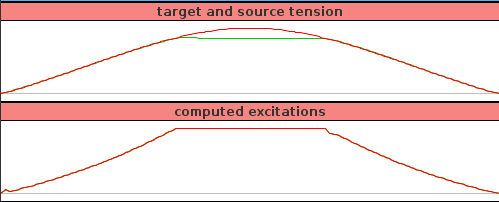
\includegraphics[]{images/InverseSpringForceProbes}
\else
   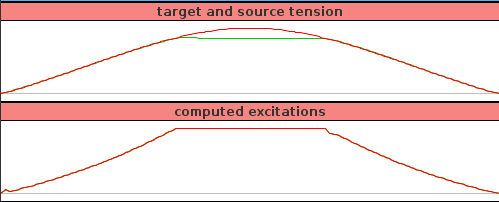
\includegraphics[width=4in]{images/InverseSpringForceProbes}
\fi
\end{center}
\caption{Probes showing the combined target and source tension (top)
and the computed excitations (bottom) for {\tt InverseSpringForce}.}
\label{InverseSpringForceProbes:fig}
\end{figure}

To run this example, select {\sf All demos > tutorial > InverseSpringForce}
from the {\sf Models} menu. The model should load and initially appear as in
Figure \ref{InverseSpringForce:fig} (left). When run, the controller computes
excitations to generate the requested tension in the passive spring; this
causes the center particle to be pulled down (Figure \ref{InverseParticle:fig},
right). Both the target-source and computed excitation probes are shown in
Figure \ref{InverseSpringForceProbes:fig}. 

For the middle third of the trajectory, the excitation values have reached
their threshold value of 1 and so are unable to deliver more force. This in
turn causes the source tension (green line) to deviate from the target tension
(red line) in the target-source probe.

%\subsection{Constraint force targets} 
%
% as indicated above, the controller can motion target components can be

\subsection{Target components}
\label{TargetComponents:sec}

As described above, when a motion or force source is added to the controller
(using methods such as {\tt addPointTarget()} or {\tt
addForceEffectorTarget()}), the controller creates and returns a target
component that is used for specifying the desired position or force
trajectory. Each target term also contains a scalar weight and a vector of
subweights, described by the properties {\sf weight} and {\sf subWeights}, all
of which have default values of 1.0. These weights are used to manage the
priority of the target within the tracking computation; the {\sf subWeights}
vector has a size equal to the number of degrees of freedom (DOF) in the target
(3 for points and 6 for frames), 
and permits fine-grained weighting for each of
the targets DOFs. The product of the weight with each subweight produces the
entries for the diagonal weighting matrix that appears in the various cost
terms for motion and force tracking (e.g., $\W_m$ for the motion tracking cost
function $\phi_m(\a)$ in (\ref{motionCostTerm:eqn}) and $\W_e$ for the force
effector cost function $\phi_e(\a)$ in (\ref{forceEffectorCostTerm:eqn})). Targets
(or specific DOFs) with higher weights will be tracked more accurately, while
weights of 0 effectively disable tracking.

Target components vary depending on the source component whose position or
force is being tracking, but each implements the interface
\javaclass[\inverse]{TrackingTarget}, which supplies
the following methods for controlling the weights and subweights and querying
the target's source component:
%
\begin{methodtable}{0.5}{0.5}
\midline
%
\methodentry
{\inverse.TrackingTarget.getSourceComp()}%
{ModelComponent getSourceComp()}%
{Returns the target's source component.}%
%
\methodentry
{\inverse.TrackingTarget.getTargetSize()}%
{int getTargetSize()}%
{Returns number of target DOFs, which equals the number of
subweights.}%
%
\methodspace{0.5em}
%
\methodentry
{\inverse.TrackingTarget.getWeight()}%
{double getWeight()}%
{Returns the target component {\sf weight} property.}%
%
\methodentry
{\inverse.TrackingTarget.setWeight(double)}%
{void setWeight(double w)}%
{Sets the target component {\sf weight} property.}%
%
\methodentry
{\inverse.TrackingTarget.getSubWeights()}%
{Vector getSubWeights()}%
{Returns the target component {\sf subweights} property.}%
%
\methodentry
{\inverse.TrackingTarget.setSubWeights()}%
{void setSubWeights(VectorNd subw)}%
{Sets the target component {\sf subweights} property.}%
%
\midline
\end{methodtable}
%

\subsection{Point and frame exciters}

In addition to muscle components, exciters may also include
\javaclass[\inverse]{PointExciter}s and
\javaclass[\inverse]{FrameExciter}s, which can be used
to apply forces directly to
\javaclass[\mech]{Point} or
\javaclass[\mech]{Frame} components. This effectively gives the inverse
controller the ability to do direct inverse simulation. These exciter
components can also assume a role similar to that of the ``reserve actuators''
used in OpenSim \cite{delp2007opensim}, augmenting a model's tracking
capabilities to account for force sources that are not explicitly supplied by
the model.

Each exciter applies a force along (or about) a single degree-of-freedom, as
specified by the enumerated types
\javaclass[\inverse]{PointExciter\$ForceDof} or
\javaclass[\inverse]{FrameExciter\$WrenchDof} and described
in the following table:

\begin{center}
\begin{tabular}{|ll|}
\hline
Enum field & Description\\
\hline
{\tt ForceDof.FX} & force along the point x axis \\
{\tt ForceDof.FY} & force along the point y axis \\
{\tt ForceDof.FZ} & force along the point z axis \\
\hline
{\tt WrenchDof.FX} & force along the frame x axis (world coordinates) \\
{\tt WrenchDof.FY} & force along the frame y axis (world coordinates) \\
{\tt WrenchDof.FZ} & force along the frame z axis (world coordinates) \\
{\tt WrenchDof.MX} & moment about the frame x axis (world coordinates) \\
{\tt WrenchDof.MY} & moment about the frame y axis (world coordinates) \\
{\tt WrenchDof.MZ} & moment about the frame z axis (world coordinates) \\
\hline
\end{tabular}
\end{center}

Point or frame exciters may be created with the following constructors:
%
\begin{methodtable}{0.6}{0.4}
\midline
%
\methodentry
{\inverse.PointExciter.PointExciter(Point,FrameDof,double}%
{PointExciter(Point point, FrameDof dof, double maxForce)}%
{Exciter for {\tt point} with {\tt dof} and {\tt maxForce}.}%
%
\methodentry
{\inverse.PointExciter.PointExciter(String,Point,FrameDof,double}%
{PointExciter(String name, Point point, FrameDof dof,\brh double maxForce)}%
{Named exciter for {\tt point} with {\tt dof} and {\tt maxForce}.}%
%
\methodspace{0.5em}%
%
\methodentry
{\inverse.FrameExciter.FrameExciter(Frame,WrenchDof,double}%
{FrameExciter(Frame frame, WrenchDof dof, double maxForce)}%
{Exciter for {\tt frame} with {\tt dof} and {\tt maxForce}.}%
%
\methodentry
{\inverse.FrameExciter.FrameExciter(Frame,WrenchDof,double}%
{FrameExciter(String name, Frame frame, WrenchDof dof, \brh double maxForce)}%
{Named exciter for {\tt frame} with {\tt dof} and {\tt maxForce}.}%
%
%\brh
\midline
\end{methodtable}
%
The {\tt maxForce} argument specifies the maximum force (or moment) that the
exciter supplies at an excitation value of 1.0.
%
\begin{sideblock}
If an exciter does not have sufficient strength to facilitate tracking, its
excitation value is likely to saturate. This can often be solved
by simply increasing the {\tt maxForce} value.
\end{sideblock}

To allow it to produce negative forces or moments along/about its specified
degree of freedom, the excitation bounds for a point or frame exciter
must be set to $[-1,1]$. The {\tt TrackingController} does this
automatically whenever a point or frame exciter is added to it.

For convenience, {\tt PointExciter} and {\tt FrameExciter} provide static
methods for creating sets of exciters to control all the translational
forces and/or moments on a given point or frame:
%
\begin{methodtable}{0.6}{0.4}
\midline
%
\methodentry
{\inverse .PointExciter.createPointExciters()}%
{ArrayList<PointExciter> createPointExciters (MechModel mech,\brh
Point point, double maxForce, boolean createNames)}%
{Create three exciters to control all forces on a point.}%
%
\methodspace{0.5em}%
\methodentry
{\inverse .FrameExciter.createFrameExciters()}%
{ArrayList<FrameExciter> createFrameExciters (\brh MechModel mech,
Frame frame, double maxForce, \brh double maxMoment, boolean createNames)}%
{Create six exciters to control all forces \& and moments on a frame.}%
%
\methodspace{0.5em}%
\methodentry
{\inverse .FrameExciter.createForceExciters()}%
{ArrayList<FrameExciter> createForceExciters (MechModel mech,\brh
Frame frame, double maxForce, boolean createNames)}%
{Create three exciters to control all forces on a frame.}%
%
\methodspace{0.5em}%
\methodentry
{\inverse .FrameExciter.createMomentExciters()}%
{ArrayList<FrameExciter> createMomentExciters (\brh MechModel mech,
Frame frame, \brh double maxMoment, boolean createNames)}%
{Create three exciters to control all moments on a frame.}%
%
%\methodspace{0.5em}%
%\brh
\midline
\end{methodtable}
%
If the (optional) {\tt mech} argument in these methods is
is non-{\tt null}, the exciters are added to
the {\tt MechModel}'s {\tt forceEffectors} list.
If the argument {\tt createNames} is {\tt true},
and the point or frame itself has a non-{\tt null} name,
then the exciter is assigned a name based on the point/frame name
and the degree of freedom.

\subsection{Example: controlling ToyMuscleArm with FrameExciters}

The {\tt InverseMuscleArm} example of Section
\ref{InverseMuscleArm:sec} can be modified to use
frame exciters in place of its muscles, allowing link forces
to be controlled directly to make the marker follow
the specified path. The modified model is
{\tt artisynth.demos.tutorial.InverseFrameExcitereArm},
and the sections of code where it differs
from {\tt InverseMuscleArm:sec} are listed below:
%
\lstset{numbers=left}
\iflatexml
%% Hack: latexml lstinputlisting doesn't handle firstline correctly
\lstinputlisting[firstline=27,lastline=37]{../../src/artisynth/demos/tutorial/InverseFrameExciterArm.java}
\else
\lstset{firstnumber={27}}
\lstinputlisting[firstline=27,lastline=37]{../../src/artisynth/demos/tutorial/InverseFrameExciterArm.java}
\lstset{firstnumber={1}}
\fi
\lstset{numbers=none}
%
%
\lstset{numbers=left}
\iflatexml
%% Hack: latexml lstinputlisting doesn't handle firstline correctly
\lstinputlisting[firstline=48,lastline=64]{../../src/artisynth/demos/tutorial/InverseFrameExciterArm.java}
\else
\lstset{firstnumber={48}}
\lstinputlisting[firstline=48,lastline=64]{../../src/artisynth/demos/tutorial/InverseFrameExciterArm.java}
\lstset{firstnumber={1}}
\fi
\lstset{numbers=none}
%
After the controller is created (lines 48-49), the muscle rest lengths are
reset, as they are for {\tt InverseMuscleArm}, but they are {\it not} added to
controller as exciters. Instead, four frame exciters are created to generate
translational forces on each link in the x-z plane, up to a maximum force of
200 (lines 61-64). These exciters are created using the method {\tt
addFrameExciter()} (lines 32-37), which creates the exciter and adds it to the
{\tt MechModel} and to the controller's exciter list.

\iflatexml\else\clearpage\fi

Instead of calling the method {\tt addFrameExciter()}, the frame exciters could have been generated using the following code fragment:
%
\begin{lstlisting}[]
   tcon.addExciters (
      FrameExciter.createForceExciters (
         myMech, myLink0, 200, /*createNames*/false));
   tcon.addExciters (
      FrameExciter.createForceExciters (
         myMech, myLink1, 200, /*createNames*/false));
\end{lstlisting}
%
This would create six exciters instead of four (three forces per link, instead
of limiting forces to x-z plane), but the additional forces would simply not be
recruited by the controller.

\begin{figure}[ht]
\begin{center}
   \iflatexml
      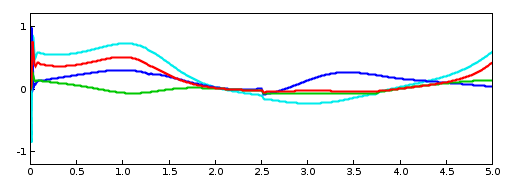
\includegraphics[]{images/InverseFrameExciterArmEx}
   \else
      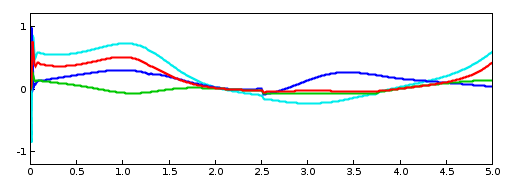
\includegraphics[width=3.25in]{images/InverseFrameExciterArmEx}
   \fi
\end{center}
\caption{Excitations computed for {\tt InverseFrameExciterArm}.}
\label{InverseFrameExciterArmEx:fig}
\end{figure}

To run this example, select {\sf All demos > tutorial > InverseFrameExciterArm}
from the {\sf Models} menu. The excitations generated by
running the model are shown in Figure \ref{InverseFrameExciterArmEx:fig}.

%\subsection{Other constraint terms}

%\subsection{Other cost terms}

\section{Tracking controller structure and settings}
\label{controllerSettings:sec}

\subsection{Controller structure}

\begin{figure}[ht]
\begin{center}
\iflatexml
   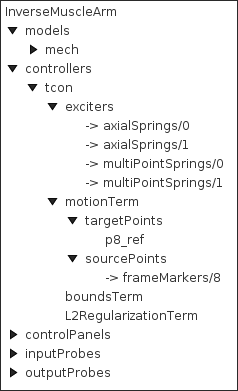
\includegraphics[]{images/TrackingControllerNavpanel}
\else
   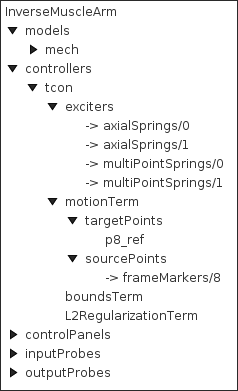
\includegraphics[width=2in]{images/TrackingControllerNavpanel}
\fi
\end{center}
\caption{Expanded navigation panel view of the tracking controller
(named {\tt "tcon"}) and all its subcomponents, for the example {\tt
InverseMuscleArm}.}
\label{TrackingControllerNavpanel:fig}
\end{figure}

The tracking controller is a composite component, which contains the exciter
list and the various cost and constraint terms as subcomponents. Some of these
components are added as needed. They include the following, as described by
their names:

\begin{description}

\item[\tt exciters]\mbox{}

A list of references to the exciters which have been added to the controller.
Note that this is a list of {\it references}; the exciters themselves exist
elsewhere in the model. Always present.

\item[\tt motionTerm]\mbox{}

The {\tt MotionTargetTerm} detailed in Section \ref{MotionTargetTerm:sec}.
Implements the motion cost term $\phi_m(\a)$ defined in
(\ref{MotionCostTerm:eqn}), and the motion tracker of
Figure \ref{trackingController:fig}.  Allocates and maintains target components
for motion sources, storing the targets in the subcomponent lists {\tt
targetPoints} and {\tt targetFrames}, and references to the sources in the
reference lists {\tt sourcePoints} and {\tt sourceFrames}. Always present.

\item[\tt forceEffectorTerm]\mbox{}

The {\tt ForceEffectorTerm} detailed in Section \ref{ForceEffectorTerm:sec}.
Implements the force effector cost term $\phi_e(\a)$ defined in
(\ref{forceEffectorCostTerm:eqn}).  Allocates and maintains target components
for force effector sources, storing then in the subcomponent list {\tt
forceTargets}. Added on demand.

\item[\tt boundsTerm]\mbox{}

Implements the actuator bounds $\a_\text{min} \le \a \le \a_\text{max}$,
where $\a_\text{min}$ and $\a_\text{max}$ are nominally $\bf 0$
and $\bf 1$. Always present.

\item[\tt L2RegularizationTerm]\mbox{}

Implements the cost term for L2 regularization
(Section \ref{L2Regularization:sec}). Added on demand.

\item[\tt dampingTerm]\mbox{}

Implements the cost term for excitation damping
(Section \ref{ExcitationDamping:sec}). Added on demand.

\end{description}

\subsection{Controller properties}
\label{ControllerProperties:sec}

The controller and its cost terms have a number of properties that can be used
to adjust the controller's behavior. They can be set interactively,
either through the inverse
controller panel created by the {\tt InverseManager} (Section
\ref{InverseControlPanel:sec}), or 
by selecting the relevant component in the navigation panel and choosing {\sf
"Edit properties ..."} from the context menu. The properties can also be set
in code, using the accessor methods supplied by their host component.  These
methods will usually be named {\tt getXxx()} and {\tt setXxx()} for
property {\sf xxx}.Properties of the tracking controller itself include:

\begin{description}

\item[active]\mbox{}

Controls whether or not the controller is active. Setting this to {\tt false}
turns the controller off. Default value is {\tt true}.

\item[normalizeCostTerms]\mbox{}

Controls whether or not the cost terms are normalized. Normalizing the terms
helps ensure that their weights (e.g., $w_m$, $w_e$, and $w_a$ in
(\ref{fullQP:eqn}) more accurately control the tradeoffs between terms.
Default value is {\tt true}.

\item[computeIncrementally]\mbox{}

Controls whether excitation values should be computed incrementally, as
described in Section \ref{IncrementalComputation:sec}.  Default value is {\tt
false}.

\item[excitationBounds]\mbox{}

Specifies the default excitation bounds for exciter components.  Default value
is $[0, 1]$.

\item[targetsVisible]\mbox{}

Controls the visibility of the motion target terms contained within the
controller, as described in Section \ref{MotionTargetRendering:sec}. Default
value is {\tt true}.

\item[configExcitationColoring]\mbox{}

If enabled, automatically configures exciters which support excitation coloring
to vary from white to red as their excitation increases
(Section \ref{ExcitationColoring:sec}). Default value is {\tt true}.

\item[probeDuration]\mbox{}

Default duration of probes managed by the 
\javaclass[\inverse]{InverseManager} class (Section \ref{InverseManager:sec}).
Default value is 1.0.

\item[probeUpdateInterval]\mbox{}

Default update interval of output probes managed by the
\javaclass[\inverse]{InverseManager} class (Section \ref{InverseManager:sec}).
Default value is -1, which means that the interval will
default to the simulation step size.

\item[useKKTFactorization]\mbox{}

Uses a more computationally expensive but possibly more accurate method to
compute the excitation response matrices matrices such as $\H_m$ and $\H_e$
(Section \ref{GeneratingExcitations:sec}). Default value is {\tt false}.

\item[maxExcitationJump]\mbox{}

Experimental property that limits the change in excitation during any time
step. Default value is {\tt false}.

\item[useTimestepScaling]\mbox{}

Experimental property which enables scaling of all the cost
terms by the simulation time step. Default value is {\tt false}.

\item[debug]\mbox{}

Enabled debugging messages. Default value is {\tt false}.

\end{description}

\subsection{Motion term properties}
\label{MotionTermProperties:sec}

The motion target term (Section \ref{MotionTargetTerm:sec}) exports a number of
properties that control motion tracking:

\begin{description}

\item[enabled]\mbox{}

Controls whether or not this term is enabled. Default value is {\tt true}.

\item[weight]\mbox{}

Specifies the weight $w_m$ of this term relative to the other cost
terms. Default value is 1.0.

\item[chaseTime]\mbox{}

Specifies the {\it chase time} $T$ used for chase control
(Section \ref{ChaseControl:sec}). Default value is 0.01.

\item[usePDControl]\mbox{}

Controls whether or not PD control is used
(Section \ref{PDControl:sec}). Default value is {\tt false}.

\item[Kp]\mbox{}

Specifies the proportional terms for PD control
(Section \ref{PDControl:sec}). Default value is 10000.

\item[Kd]\mbox{}

Specifies the derivative terms for PD control
(Section \ref{PDControl:sec}). Default value is 100.

\item[legacyControl]\mbox{}

Controls whether or not legacy control is used.
Default value is {\tt false}.

\end{description}

\subsection{Properties for other cost terms}

All other cost terms, including the L2 regularization (Section
\ref{L2Regularization:sec}), export the following properties:

\begin{description}

\item[enabled]\mbox{}

Controls whether or not the term is enabled. Default value is {\tt true}.

\item[weight]\mbox{}

Specifies the weight of this term relative to the other cost terms. Default
value is 1.0.

\end{description}

\section{Managing probes and control panels}
\label{InverseManager:sec}

The tracking controller package provides the helper class
\javaclass[\inverse]{InverseManager} to aid with the
creation of probes and control panels that are useful in for inverse simulation
applications. The functionality provided by {\tt InverseManager} is described
in this section, and additional documentation may be found in its
\javaclassAlt{\inverse.InverseManager}{API documentation}.

\subsection{Inverse simulation probes}
\label{InverseManagerProbes:sec}

\begin{table}[h]
\begin{center}
\begin{tabular}{|llll|}
\hline
ProbeID & I/O type & Probe name & Default filename \\
\hline
{\tt TARGET\_POSITIONS} & input & {\tt "target positions"} &
{\tt target\_positions.txt} \\
{\tt INPUT\_EXCITATIONS} & input & {\tt "input excitations"} &
{\tt input\_excitations.txt} \\
{\tt TRACKED\_POSITIONS} & output & {\tt "tracked positions"} &
{\tt tracked\_positions.txt} \\
{\tt SOURCE\_POSITIONS} & output & {\tt "source positions"} &
{\tt source\_positions.txt} \\
{\tt COMPUTED\_EXCITATIONS} & output & {\tt "computed excitations"} &
{\tt computed\_excitations.txt} \\
\hline
\end{tabular}
\end{center}
\caption{Probe types, names, and default file names associated 
with {\tt ProbeID}.}
\label{ProbeData:tab}
\end{table}

{\tt InverseManager} contains static methods that support the creation and
management of a variety of probes related to inverse simulation. These probes
are defined by the enumerated type
\javaclass[\inverse]{InverseManager\$ProbeID},
which includes the following identifiers:

\begin{description}

\item[{\tt TARGET\_POSITIONS}]\mbox{}

An input probe which provides a trajectory $\x_t(t)$ for all motion
targets. Its input values are attached to the {\sf position} property (3 values)
of each point target and the {\sf position} and {\sf orientation} properties of
each frame target (7 values), in the order the targets appear in the
controller.

\item[{\tt INPUT\_EXCITATIONS}]\mbox{}

An input probe which provides input excitation values for all the controller's
exciters, in the order they appear in the controller. This probe can be used
for testing purposes, in order to see what trajectory can be expected to arise
from a given excitation input.

\item[{\tt TRACKED\_POSITIONS}]\mbox{}

An output probe which records the positions of all motion targets as they are
set by the controller. Its output values are extracted from the same component
properties used by {\tt TARGET\_POSITIONS}.

\item[{\tt SOURCE\_POSITIONS}]\mbox{}

An output probe which records that actual position trajectory $\x(t)$ followed
by all motion sources. Its output values are extracted from the same component
properties used by {\tt TARGET\_POSITIONS}.

\item[{\tt INPUT\_EXCITATIONS}]\mbox{}

An output probe which records the computed excitation values for all the
controller's exciters, in the order they appear in the controller.

\end{description}

Each of these probes is associated with both a name and a default file name
(Table \ref{ProbeData:tab}), where the default file name may be assigned if
another file path is not explicitly specified.

\begin{sideblock}
When a default file name is used, it is assumed to be relative to the ArtiSynth
working folder, as described in Section \ref{Probes:sec}.
\end{sideblock}

These probes may be created, for a given tracking controller, with the
following (static) {\tt InverseManager} methods:
%
\begin{methodtable}{0.6}{0.4}
\midline
%
\methodentry
{\inverse.InverseManager.createInputProbe()}%
{NumericInputProbe createInputProbe (TrackingController tcon\brh
ProbeID pid, String filePath, double start, double stop)}%
{Create input probe specified by {\tt pid}.}%
%
\methodspace{0.5em}%
\methodentry
{\inverse.InverseManager.createOutputProbe()}%
{NumericOutputProbe createOutputProbe (TrackingController tcon\brh
ProbeID pid, String filePath, double start, double stop, \brh double interval)}%
{Create output probe specified by {\tt pid}.}%
%
%\methodspace{0.5em}%
%\brh
\midline
\end{methodtable}
%
Here {\tt pid} specifies the probe type, {\tt filePath} an (optional) file
path, {\tt start} and {\tt stop} the start and stop times, and {\tt interval}
the output probe update interval.

Created probes may be added to the application root model as needed.

Most of the examples above use {\tt createOutputProbe()} to create a computed
excitations probe. In {\tt InverseMuscleFem}
(Section \ref{InverseMuscleFem:sec}), the two output probes used to display the
tracked position and orientation of {\tt myFrame}, created at lines (42-51),
{\it could} be replaced by a single probe of type {\tt SOURCE\_POSITIONS},
using a code fragment like this:
%
\begin{lstlisting}[]
      NumericOutputProbe sourceProbe = InverseManager.createOutputProbe (
         tcon, ProbeID.SOURCE_POSITIONS, /*fileName=*/null,
         startTime, stopTime, /*interval=*/-1);
      addOutputProbe (sourceProbe);
\end{lstlisting}
%
Likewise, a probe showing the target position and orientation, for purposes of
comparing it against {\tt SOURCE\_POSITIONS} and evaluating the tracking error,
could be created using
%
\begin{lstlisting}[]
      NumericOutputProbe trackedProbe = InverseManager.createOutputProbe (
         tcon, ProbeID.TRACKED_POSITIONS, /*fileName=*/null,
         startTime, stopTime, /*interval=*/-1);
      addOutputProbe (trackedProbe);
\end{lstlisting}
%
For both these method calls, the source and target components ({\tt myFrame}
and {\tt target} in the example) are automatically located within the tracking
controller.

\begin{sideblock}
One reason to create a {\tt TRACKED\_POSITIONS} probe, instead of comparing
{\tt SOURCE\_POSITIONS} directly against the trajectory input probe, is that
the former is guaranteed to have the same number of data points as {\tt
SOURCE\_POSITIONS}, whereas a trajectory probe, being an input probe, may
not. Moreover, if the trajectory is being produced using a controller,
a trajectory probe may not even exist.
\end{sideblock}

For convenience, {\tt InverseManager} also provides methods to add a complete
set of default probes to the root model:
%
\begin{methodtable}{0.6}{0.4}
\midline
%
\methodentry
{\inverse.InverseManager.addProbes()}%
{void addProbes (RootModel root, TrackingController tcon,\brh
double duration, double interval)}%
{Add default probes to {\tt root}.}%
%
\methodspace{0.5em}%
\methodentry
{\inverse.InverseManager.resetProbes()}%
{void resetProbes (RootModel root, TrackingController tcon,\brh
double duration, double interval)}%
{Clear probes and add default probes to {\tt root}.}%
%
%\methodspace{0.5em}%
%\brh
\midline
\end{methodtable}
%
{\tt addProbes()} creates a {\tt COMPUTED\_EXCITATIONS} probe and an {\tt
INPUT\_EXCITATIONS} probe, with the latter deactivated by default.  If the
controller has any motion targets, it will also create {\tt TARGET\_POSITIONS},
{\tt TRACKED\_POSITIONS} and {\tt SOURCE\_POSITIONS} probes.  Probe start times
are set to 0, stop times are set to {\tt duration}, and the output probe update
interval is set to {\tt interval}, with -1 causing the interval to default to
the simulation step size. Probe file names are set to the default file names
described in Table \ref{ProbeData:tab}.  Since these file names are relative,
the files themselves are assumed to exist in the ArtiSynth working folder, as
described in Section \ref{Probes:sec}. If the file for an input probe actually
exists, it is used to initialize the probe's data; otherwise, the probe data is
initialized to 0 and the probe is deactivated.

{\tt resetProbes()} removes all existing probes and then behaves identically to
{\tt addProbes()}.


{\tt InverseManager} also supplies methods to locate and adjust the probes that
it has created:
%
\begin{methodtable}{0.65}{0.35}
\midline
%
\methodentry
{\inverse.InverseManager.findInputProbe()}%
{NumericInputProbe findInputProbe (RootModel root, ProbeID pid)}%
{Find specified input probe.}%
%
\methodentry
{\inverse.InverseManager.findOutputProbe()}%
{NumericOutputProbe findOutputProbe (RootModel root, ProbeID pid)}%
{Find specified output probe.}%
%
\methodentry
{\inverse.InverseManager.findProbe()}%
{Probe findProbe (RootModel root, ProbeID pid)}%
{Find specified input or output probe.}%
%
\methodspace{0.5em}%
%
\methodentry
{\inverse.InverseManager.setInputProbeData()}%
{boolean setInputProbeData (RootModel root, \brh ProbeID pid,
double[] data, double timeStep)}%
{Set input probe data.}%
%
\methodspace{0.5em}%
\methodentry
{\inverse.InverseManager.setProbeFileName()}%
{boolean setProbeFileName (RootModel root, \brh ProbeID pid,
String filePath)}%
{Set probe file path.}%
%
%\brh
\midline
\end{methodtable}
%
The {\tt findProbe()} methods search for the probe specified by {\tt pid}
within a root model, using the probe's file name (Table \ref{ProbeData:tab}) as
a search key. The method {\tt setInputProbeData()} searches for a specified
probe, and if it is found, sets its data using the probe's 
\javamethodAlt{artisynth.core.probes.NumericInputProbe.setData(,)}{%
setData(double[],double)}
method and returns {\tt true}. Likewise, {\tt setProbeFileName()} searches for
a specified probe and sets its file path.

\begin{sideblock}
Since probes maintained by {\tt InverseManager} use probe names as a search
key, care should be taken to ensure that these names do not conflict with those
of other application probes.
\end{sideblock}

\subsection{Example: using {\tt InverseManager} probes}

The example {\tt InverseMuscleArm} (Section \ref{InverseMuscleArm:sec}) has
been configured for use with the {\tt InverseManager} by setting its working
folder to {\tt inverseMuscleArm} located beneath its source folder.  If instead
of creating the target and output excitations probes (lines 34-52), {\tt
addProbes()} is simply called at the end of the {\tt build()} method (after the
working folder has been set), as in
%
\begin{lstlisting}[]
      // set working folder for probe files
      ArtisynthPath.setWorkingFolder (
         new File (PathFinder.getSourceRelativePath (this, "inverseMuscleArm")));
      InverseManager.addProbes (this, tcon, 5.0, -1);
\end{lstlisting}
%
then a set of probes will be created as shown in
Figure \ref{InverseMuscleArmProbes:fig}. The tracing probes ({\tt "target
tracing"} and {\tt "source tracing"}) are still present, in addition to five
default probes. {\tt TARGET\_POSITIONS} and {\tt INPUT\_EXCITATIONS} are
expanded to show the data that has been automatically loaded from the files
{\tt target\_positions.txt} and \pdfbreak 
{\tt input\_excitations.txt} located in the
working folder. By default, the former probe is enabled and the latter is
disabled. If the model is run, inverse simulation will proceed as before.

\begin{figure}[ht]
\begin{center}
\iflatexml
   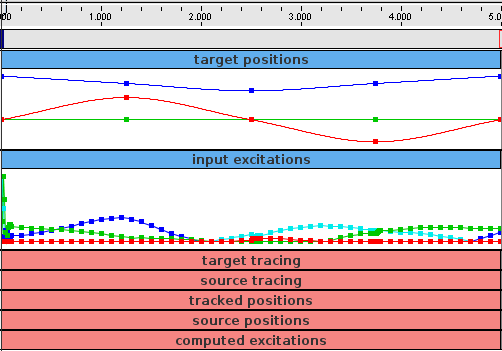
\includegraphics[]{images/InverseMuscleArmProbes}
\else
   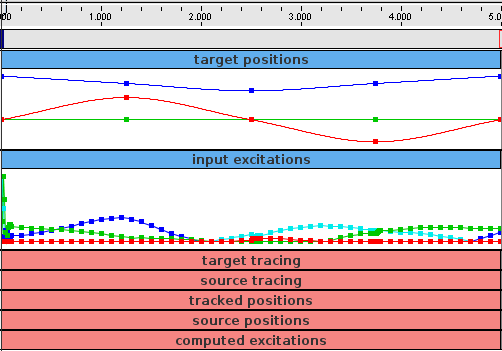
\includegraphics[width=4in]{images/InverseMuscleArmProbes}
\fi
\end{center}
\caption{{\tt InverseMuscleArm} probes with original tracing
probes and default probes.}
\label{InverseMuscleArmProbes:fig}
\end{figure}

After loading the probes, the application {\it could} disable the tracking
controller and enable the input excitations:
%
\begin{lstlisting}[]
      // set working folder for probe files
      ArtisynthPath.setWorkingFolder (
         new File (PathFinder.getSourceRelativePath (this, "inverseMuscleArm")));
      InverseManager.addProbes (this, tcon, 5.0, -1);
      tcon.setActive (false);
      InverseManager.findProbe (this, ProbeID.INPUT_EXCITATIONS).setActive (true);
\end{lstlisting}
%
This will cause the simulation to run ``open loop'' in response to the
excitations. However, because the input excitations are slightly different than
those that were computed by the controller, there is a now a considerable
tracking error (Figure \ref{InverseMuscleArmError:fig}, left). 

After the open loop run, one can save the resulting {\tt SOURCE\_POSITIONS}
probe, which will write the file \pdfbreak 
{\tt "target\_positions.txt''} into the
working folder. This can then be used to generate a new target trajectory, by
copying it to {\tt "target\_positions.txt"}. If the model is reloaded, the new
trajectory will now appear in the {\tt TARGET\_POSITIONS} probe
(Figure \ref{InverseMuscleArmProbesNew:fig}). Deactivating
the {\tt INPUT\_EXCITATIONS} probe and reactivating the tracking
controller will cause this new trajectory to be tracked properly
(Figure \ref{InverseMuscleArmError:fig}, right). 

In ways such as this, the probes may be used to examine the behavior and
performance of the tracking controller.

\begin{figure}[ht]
\begin{center}
\begin{tabular}{cc}
   \iflatexml
      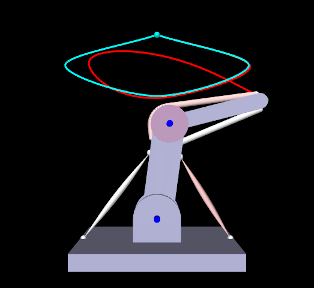
\includegraphics[]{images/InverseMuscleArmError}
      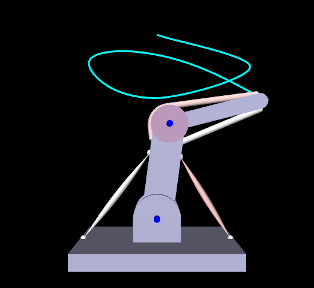
\includegraphics[]{images/InverseMuscleArmFixed}
   \else
      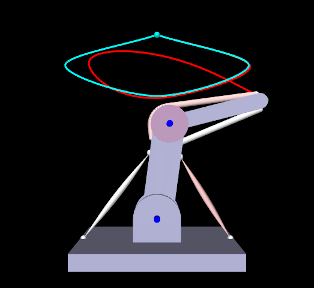
\includegraphics[width=3in]{images/InverseMuscleArmError}
      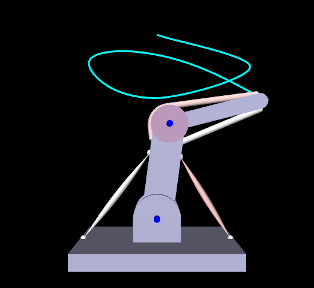
\includegraphics[width=3in]{images/InverseMuscleArmFixed}
   \fi
\end{tabular}
\end{center}
\caption{Left: {\tt InverseMuscleFem} when run open loop with excitations
loaded from {\tt "input\_excitations.txt"}. Right: model run
with inverse simulation, using new targets generated by the
open loop run.}
\label{InverseMuscleArmError:fig}
\end{figure}

\begin{figure}[ht]
\begin{center}
\iflatexml
   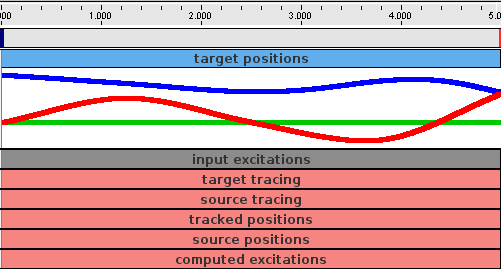
\includegraphics[]{images/InverseMuscleArmProbesNew}
\else
   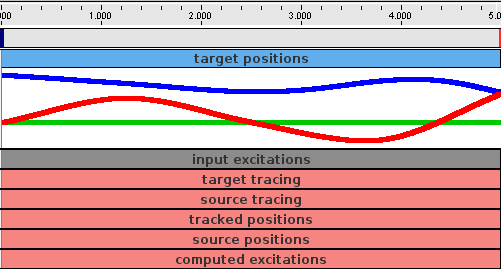
\includegraphics[width=4in]{images/InverseMuscleArmProbesNew}
\fi
\end{center}
\caption{{\tt InverseMuscleArm} probes with new target trajectory copied
from the open loop run.}
\label{InverseMuscleArmProbesNew:fig}
\end{figure}


\subsection{Inverse control panel}
\label{InverseControlPanel:sec}

{\tt InverseManager} also provide methods to create and manage an {\it inverse
control panel}, which allows interactive editing of the properties of the
tracking controller and its various cost terms, as described in Section
\ref{controllerSettings:sec}. Applications can create an instance of this 
panel in their {\tt build()} method, as the {\tt InverseMuscleArm} example
(Section \ref{InverseMuscleArm:sec}) does at line 65:
%
\begin{lstlisting}[]
      InverseManager.addInversePanel (this, tcon);
\end{lstlisting}
%
The panel is automatically configured to display the properties of the cost
terms with which the controller is currently configured. Figure
\ref{InverseControlPanel:fig} shows the panel for {\tt InverseManager}.

\begin{figure}[ht]
\begin{center}
\iflatexml
   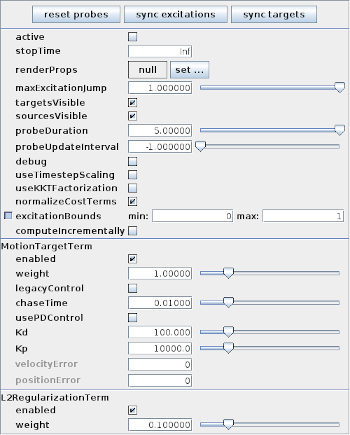
\includegraphics[]{images/InverseControlPanel}
\else
   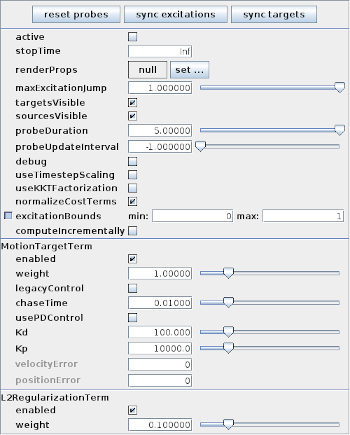
\includegraphics[width=3in]{images/InverseControlPanel}
\fi
\end{center}
\caption{Inverse control panel created for the {\tt InverseMuscleArm} demo.}
\label{InverseControlPanel:fig}
\end{figure}

The following methods are supplied by {\tt InverseManager()} to manage inverse
control panels:
%
\begin{methodtable}{0.6}{0.4}
\midline
%
\methodentry
{\inverse.InverseManager.createInversePanel()}%
{ControlPanel createInversePanel (TrackingController tcon)}%
{Create inverse control panel for {\tt tcon}.}%
%
\methodentry
{\inverse.InverseManager.addInversePanel()}%
{ControlPanel createInversePanel (RootModel root, \brh TrackingController tcon)}%
{Create and add inverse control panel to {\tt root}.}%
%
\methodentry
{\inverse.InverseManager.findInversePanel()}%
{ControlPanel findInversePanel (RootModel root)}%
{Find inverse control panel in {\tt root}.}%
%
%\methodspace{0.5em}%
%\brh
\midline
\end{methodtable}
%

At the top of the inverse panel are three buttons: {\sf "reset probes"}, {\sf
"sync excitations"}, and {\sf "sync targets"}. The first uses {\tt
InverseManager.resetProbes()} to clear all probes and recreate the default
probes, using the duration and update interval specified by the tracking
controller properties {\sf probeDuration} and {\sf probeUpdateInterval}.  The
second button copies the contents of the {\tt COMPUTED\_EXCITATIONS} probe into
the {\tt INPUT\_EXCITATIONS} probe. If this is done after excitations have been
computed, then running the simulation again with the controller deactivated and
{\tt INPUT\_EXCITATIONS} activated should produce an identical motion.  The
third button copies the contents of the {\tt SOURCE\_POSITIONS} probe into the
{\tt TARGET\_POSITIONS}. This can be used to verify that a source trajectory
created open loop with a prescribed set of input excitations can in fact be
tracked by the controller.

The probe copy methods used by the ``sync'' buttons are also available
to the application code:
%
\begin{methodtable}{0.45}{0.55}
\midline
\methodentry
{\inverse.InverseManager.syncTargetProbes()}%
{boolean syncTargetProbes (RootModel root)}%
{Copy {\tt SOURCE\_POSITIONS} into {\tt TARGET\_POSITIONS}.}%
%
\methodentry
{\inverse.InverseManager.syncExcitationProbes()}%
{boolean syncExcitationProbes (RootModel root)}%
{Copy {\tt COMPUTED\_EXCITATIONS} into {\tt INPUT\_EXCITATIONS}.}%
%
%\methodspace{0.5em}%
%\brh
\midline
\end{methodtable}

\section{Caveats and limitations}

Use of the inverse controller is subject to some caveats.

\begin{itemize}

\item Tracked components must be dynamic, in that their
motion is controlled by forces. This means that their {\sf dynamic} property
must be set to {\tt true} or they must be attached to other bodies that are
dynamic.

\item The algorithm which computes the excitations currently
has a complexity $O(n^3)$ in the number of excitations $n$.  This is due both
to the use of numeric differentiation for determining excitation response
matrices such as $\H_m$ and $\H_e$ (Section
\ref{GeneratingExcitations:sec}), and also the fact that the QP solver
is at present a dense solver. This means that applications with large numbers
of excitations may require considerably longer to simulate than those with
fewer excitations.

\item The controller is not designed to work with
unilateral constraints (the most common examples of which are constraint-based
contact and joint limits). For models containing these behaviors, inverse
simulation may produce excitations that jump around erratically.  In the case
of collisions, one solution may be to use force-based collisions, implemented
with either
\javaclass[\mech]{PointPlaneForce} or
\javaclass[\mech]{PointMeshForce}, as described in Section
\ref{OtherPointForces:sec}. Setting these components to
use a quadratic force function may improve performance even more.  Another
possible solution, for any kind of unilateral constraint, may be to make it
compliant (Sections \ref{JointCompliance:sec}
and \ref{ContactRegularization:sec}), since this has the same effect as making
the constraint force-based.

\item Prescribed motion trajectories may need to be sufficiently
smooth the avoid large transient excitations, particularly at the start and end
of motions when velocities transition from and to 0. Transient effects are
often more pronounced for models where inertial effects are high.  Cubic
interpolation is useful for creating smoother trajectories, particularly with a
limited number of data points. It may also be necessary to explicitly smooth an
input trajectory with additional points.

In the {\tt InverseMuscleArm} example, there is a noticeably transient at the
start (Figure \ref{InverseMuscleArmL2:fig}, left). Increasing the L2
regularization weight reduces the transient amplitude but spreads it out over a
longer time (Figure \ref{InverseMuscleArmL2:fig}, right), at the expense of
tracking accuracy.

\end{itemize}

%
\ifdefined\maindoc
\else
\end{document}
\fi
